% paper_arxiv_draft.tex
% From Tokens to Energy: The Cost of Replacing Human Engineering with AI
% arXiv-format LaTeX version
% Generated from paper_arxiv_draft.md

\documentclass{article}
\usepackage{PRIMEarxiv}         % arXiv preprint style (Times, fancyhdr, 6.5in text)


%% ── Packages ─────────────────────────────────────────────────────────────
\usepackage{array}
% \usepackage{booktabs}
\usepackage[utf8]{inputenc}
\usepackage[T1]{fontenc}
% lmodern omitted: cs_2025 sets Times Roman (ptm/phv)
\usepackage{microtype}
% geometry omitted: PRIMEarxiv sets 6.5in × 9in layout internally
\usepackage{amsmath,amssymb}
\usepackage{booktabs}           % professional tables
\usepackage{longtable}
\usepackage{array}
\usepackage{tabularx}
\usepackage[table]{xcolor}
\usepackage{graphicx}
\usepackage{hyperref}
\usepackage[capitalize,noabbrev]{cleveref}
\usepackage{tcolorbox}          % callout boxes
\tcbuselibrary{skins,breakable}
\usepackage{listings}           % code blocks
\usepackage{lstautogobble}
\usepackage{setspace}
\usepackage{parskip}
\usepackage{enumitem}
\usepackage{caption}
\usepackage{subcaption}
\usepackage{pdflscape}
\usepackage{natbib}             % PRIMEarxiv does not load natbib
% fontawesome5 omitted: crashes tectonic/XeTeX (use text fallback below)

%% ── Custom commands ──────────────────────────────────────────────────────
% Citation quality flags
\newcommand{\PRIMARY}{\textbf{[PRIMARY]}}
\newcommand{\SECONDARY}{\textbf{[SECONDARY]}}
\newcommand{\ESTIMATE}{\textbf{[ESTIMATE]}}
\newcommand{\VERIFY}{\textcolor{red}{\textbf{[VERIFY]}}}

%% ── tcolorbox styles ─────────────────────────────────────────────────────
\tcbset{
  warningbox/.style={
    enhanced,
    colback=yellow!10,
    colframe=orange!80!black,
    fonttitle=\bfseries,
    title={$\blacktriangleright$\ Note},
    breakable
  },
  keyresult/.style={
    enhanced,
    colback=blue!5,
    colframe=blue!60!black,
    fonttitle=\bfseries,
    title={Key Result},
    breakable
  }
}

%% ── lstlisting style ─────────────────────────────────────────────────────
\lstset{
  basicstyle=\small\ttfamily,
  breaklines=true,
  frame=single,
  autogobble=true,
  xleftmargin=2em,
  xrightmargin=2em
}

%% ── Hyperref setup ───────────────────────────────────────────────────────
\hypersetup{
  colorlinks=true,
  linkcolor=blue!70!black,
  citecolor=green!50!black,
  urlcolor=blue!70!black,
  pdftitle={From Tokens to Energy: The Cost of Replacing Human Engineering with AI},
  pdfauthor={Draft v0.1},
  pdfsubject={AI infrastructure, labor substitution, token economics}
}

%% ── Title block ──────────────────────────────────────────────────────────
\title{%
  \textbf{Tokenizing Labor: A Probabilistic Evaluation for Compute and Energy Requirements of AI Software Engineering Substitution}
  % \\[0.5em]
  % \large\textit{Quantifying the Infrastructure Imperative: Token Demand, Energy Consumption,
  % and Market Opportunities in the AI-Driven Engineering Transition}
}

\author{%
  Ge Zhang \\
  Department of Energy Science \& Engineering \\
  Stanford University \\
  \texttt{gmzhang@stanford.edu}
  % \And
  % Claude Sonnet 4.6 (Claude Code) \\
  % Anthropic, PBC \\
  % \texttt{claude-code@anthropic.com}
  \And
  Jingru Cheng \\
  Department of Energy Science \& Engineering \\
  Stanford University \\
  \texttt{cjr63@stanford.edu}
  \And
  Zitong Huang \\
  Department of Energy Science \& Engineering \\
  Stanford University \\
  \texttt{zthuang@stanford.edu}
  \And
  Anthony R. Kovscek \\
  Department of Energy Science \& Engineering \\
  Stanford University \\
  \texttt{kovscek@stanford.edu}
}

\date{}

% ─────────────────────────────────────────────────────────────────────────────
\begin{document}
\maketitle

% -- check the data sources
% \noindent\small\textit{All data quality flags: \PRIMARY{} = directly citable;
% \SECONDARY{} = citable with caveat; \ESTIMATE{} = derived/illustrative;
% \VERIFY{} = requires primary source before submission.}

\vspace{1em}
\hrule
\vspace{1em}

% ─────────────────────────────────────────────────────────────────────────────

% If AI agents substitute for a meaningful fraction of software engineering labor, what physical infrastructure, energy demand, and capital investment are required to operate that replacement workforce?

\begin{abstract}
Artificial intelligence (AI) systems are demonstrating increasing capability at software engineering tasks, raising the concern of large-scale substitution of human engineering labor by AI inference. However, the energy demand and cost has not yet been systematic evaluated from a bottom-up logic. To delineate the substitution map, we construct a quantitative evaluation model linking engineering workforce to AI compute infrastructure requirements, using token consumption linked with energy cost across a spectrum of AI human resource substitution scenarios. Firstly, the \emph{token} is taken as the analytical bridge between labor economics (FTE-hours, compensation) and computational economics (FLOP/s, kilowatt-hours). Using a five-category task taxonomy to bound substitutability, token consumption evaluation experiment from SWE coding benchmarks, and hardware throughput benchmarks for current AI tools, we derive the compute and energy requirements for replacing 10\%, 30\%, 50\%, 70\% of the software engineering FTE under fully software agentic AI deployment. 
% provide some numbers here ...
% However, the binding constraints on AI engineering deployment are not economic but operational: current agentic capability (SWE-bench resolution rate), institutional adoption friction, and grid interconnection timelines of 2--5 years for large loads. 

We map the resulting opportunity and tasks across energy companies, data center developers, equipment suppliers, and capital markets instruments, and identify serval priorities on fast-track grid interconnection for AI-critical loads, pre-funded engineering workforce transition programs, and mandatory AI inference carbon accounting.



\end{abstract}

\vspace{0.5em}
\noindent\textbf{Keywords:} Artificial Intelligence, Token Consumption, Energy, AI Infrastructure, Labor Substitution

% \vspace{0.3em}
% \noindent\textbf{arXiv subject classifications:} cs.AI (Artificial Intelligence);
% econ.GN (General Economics); cs.CY (Computers and Society)

% \vspace{0.3em}
% \noindent\textbf{MSC classes:} 91B38 (Production theory, theory of the firm);
% 68T01 (General topics in artificial intelligence)

\vspace{1em}
\hrule

% % ─────────────────────────────────────────────────────────────────────────────
% \tableofcontents
% \newpage

% ─────────────────────────────────────────────────────────────────────────────

\section{Introduction and Motivation}
\label{sec:introduction}

Energy availability has historically constrained every major wave of technological transformation. From industrial mechanization and electrification to modern cloud computing, sustained productivity growth has ultimately depended on the availability of physical infrastructure capable of supporting new forms of production. Artificial intelligence is increasingly emerging as a general-purpose technology with the potential to reshape large segments of the global economy. However, unlike previous digital technologies that primarily facilitated communication, information retrieval, or process automation, modern AI systems directly convert electrical energy into economically productive cognitive work through large-scale inference computation. As AI agents become capable of performing increasingly sophisticated professional tasks especially in software industry, understanding their infrastructure requirements, energy consumption, and operating costs becomes essential for evaluating the practical limits and economic implications of AI deployment.

This challenge has become particularly important as governments, cloud providers, and technology firms commit hundreds of billions of dollars to AI infrastructure expansion. Recent projections from the International Energy Agency suggest that AI deployment could become a major driver of future data-center electricity demand growth \citep{iea2025energyai}. Parallel analyses from industry and national laboratories similarly highlight increasing concerns regarding GPU supply, datacenter construction, electrical capacity constraints, and the long-term sustainability of large-scale AI deployment \citep{lbnl2024datacenterenergy}. Despite growing attention to AI energy consumption, however, existing infrastructure forecasts often estimate future demand from projected hardware deployment or aggregate model usage trends rather than from the underlying activities AI systems are expected to perform.

% U.S. data center electricity: 176 TWh (2023), 183 TWh (2024), projected 325--580 TWh by 2028 (6.7--12\% of total U.S. electricity); baseline 58 TWh in 2014

Among the many occupations potentially affected by AI, software engineering represents a particularly important case study. Software development constitutes one of the largest and most economically valuable categories of high-skilled knowledge work in the global economy. The United States employed approximately 1.89 million software developers in 2024, with a median annual wage of \$133,080 according to the U.S. Bureau of Labor Statistics Occupational Employment and Wage Statistics (OEWS) program \citep{bls2024oes}. The occupation is projected to grow by 17\% between 2024 and 2034, substantially faster than the average across all occupations \citep{bls2024ooh}. Globally, the professional software developer population reached approximately 20.8 million in 2025 according to \citet{jetbrains2025survey}, while broader estimates place the worldwide developer population between 27 and 29 million individuals \citep{evans2025developers}. Consequently, even partial substitution of software-engineering labor by AI systems would affect a workforce measured in tens of millions of workers and potentially redirect a substantial quantity of economic activity from human labor toward computational infrastructure.

Recent advances in large language models and autonomous agent systems suggest that such substitution is increasingly technically feasible. Unlike previous waves of automation that primarily mechanized physical execution while leaving human cognition as the central coordinating function, frontier AI systems increasingly target cognitive and linguistic components of professional work itself. Modern software-engineering agents are capable of generating code, planning execution strategies, invoking external tools, navigating repositories, interpreting compiler feedback, executing debugging loops, and iteratively refining software artifacts with limited direct human intervention \citep{santos2026decoding, hosseini2025roleofai, wang2025agentic, patil2025bfcl}. As of early 2026, frontier software-engineering agents routinely achieve resolution rates exceeding 70\% on \textit{SWE-bench Verified}, a widely used benchmark evaluating repository-level software maintenance and bug-fixing tasks under executable testing conditions \citep{swebench2026}. Although benchmark performance does not directly imply occupational replacement, these results establish a meaningful lower bound on the technical feasibility of software-engineering automation.

At the same time, rapid enterprise adoption is transforming AI agents from experimental software tools into economically significant consumers of computational resources. Large organizations increasingly report that token consumption, rather than model licensing alone, has become a major operational cost. For example, Uber disclosed that widespread adoption of AI coding assistants exhausted its annual AI tooling budget within the first four months of 2026, prompting executives to explicitly evaluate the trade-off between token consumption, infrastructure expenditure, and engineering productivity. Similar concerns have emerged across enterprise deployments as organizations shift from measuring AI adoption to quantifying its economic return.

This trend introduces a fundamental analytical challenge. Labor economics traditionally measures productive activity using units such as workers, hours, and compensation, whereas AI systems consume tokens, floating-point operations, GPU-hours, and electricity. Existing literature has extensively examined labor substitution \citep{autor2003skill, acemoglu2022tasks}, foundation-model scaling \citep{kaplan2020scaling, hoffmann2022chinchilla}, large language model capabilities \citep{brown2020gpt3, bommasani2021foundation}, autonomous agents \citep{wang2025agentic, patil2025bfcl, rothschild2025agentic}, and AI energy demand \citep{iea2025energyai, lbnl2024datacenterenergy}. However, these research directions remain largely disconnected. Studies of AI-driven labor substitution rarely quantify the computational infrastructure required to support large-scale deployment, while infrastructure and energy analyses seldom identify the categories of human work that ultimately generate inference demand. Consequently, there remains no unified framework that translates software-engineering labor into token demand, GPU requirements, and electricity consumption.

This disconnect is particularly important because recent evidence suggests that autonomous AI systems may exhibit fundamentally different computational characteristics than traditional human-in-the-loop AI applications. Empirical studies of agentic software-engineering systems indicate that autonomous coding workflows can consume orders of magnitude more tokens than conventional copilot-style interactions \citep{salim2026tokenomics, bai2026agent}. While interactive coding assistants may operate on the order of $10^5$ tokens per engineer per day, fully autonomous software-engineering agents can consume on the order of $10^6$--$10^7$ tokens for complex repository-level tasks. Consequently, large-scale labor substitution may generate disproportionately larger increases in compute demand and electricity consumption than implied by conventional AI adoption metrics.

This study argues that the key missing link connecting labor work, AI capability, infrastructure planning, and energy systems is the \textbf{token}. Tokens constitute the atomic unit of language-model computation and provide a measurable bridge between human cognitive labor and physical infrastructure requirements. Engineering activities can be translated into token demand; token demand determines inference throughput requirements; inference throughput determines GPU deployment, electrical power consumption, and operating cost. By expressing software-engineering labor in token terms, it becomes possible to quantitatively connect occupational-scale AI adoption to the infrastructure and energy systems required to sustain it.

Accordingly, this paper develops a bottom-up framework that links software-engineering labor substitution to token demand, GPU infrastructure requirements, electricity consumption, and deployment cost. The central scenario modeled throughout the paper assumes some content of effective software-engineering labor substitution, broadly consistent with accelerated AI deployment scenarios discussed in recent workforce analyses \citep{mckinsey2024future}. Rather than asking only whether AI systems can replace portions of software-engineering labor, we examine a complementary infrastructure question:

\begin{quote}
\textit{How much computational infrastructure, electrical energy, and economic expenditure are required to substitute for software-engineering labor at meaningful scale?}
\end{quote}

By answering this question, the paper contributes a unified framework connecting labor substitution, tokenized inference demand, compute infrastructure, and energy consumption. In doing so, it reframes AI automation not only as a labor-market phenomenon, but also as a problem in infrastructure economics, energy systems planning, and the physical scalability of artificial intelligence.


% ─────────────────────────────────────────────────────────────────────────────

\section{Stochastic Labor-to-Infrastructure Modeling Framework}
\label{sec:Modeling}

Figure~\ref{fig:01_modeling} illustrates the modeling framework used throughout this study. The framework begins with an assumed level of software-engineering labor substitution, expressed in FTE-equivalent terms, and progressively translates that labor demand into token consumption, inference throughput, GPU infrastructure requirements, electricity consumption, and economic cost. The central premise of the framework is that tokens provide a measurable bridge between human cognitive labor and physical AI infrastructure. By modeling software-engineering work in token terms, labor-substitution scenarios can be systematically mapped to compute demand, energy consumption, and infrastructure deployment requirements. The framework also explicitly incorporates major sources of uncertainty, including substitution rates, token intensity, model architecture, hardware performance, agent retry behavior, infrastructure utilization, and datacenter efficiency.

\begin{figure}
    \centering
    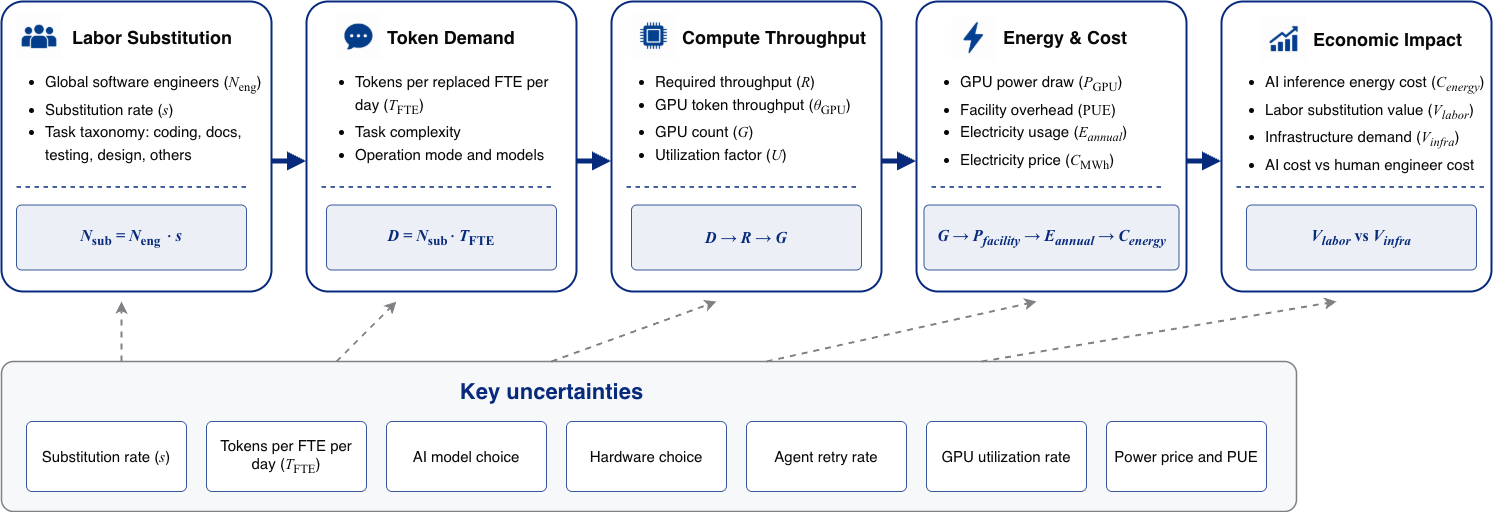
\includegraphics[width=1.0\linewidth]{figures/Fig_1_modeling_framework.png}
    \caption{Bottom-up labor-to-infrastructure modeling framework for AI software-engineering substitution. The framework converts FTE-equivalent software-engineering labor into token demand, inference throughput, GPU infrastructure requirements, electricity consumption, and economic cost. Tokens serve as the intermediate accounting unit linking cognitive labor to physical compute and energy systems. The lower panel summarizes major uncertainty drivers affecting labor substitution, token intensity, model and hardware selection, agent behavior, infrastructure utilization, and datacenter efficiency.}
    \label{fig:01_modeling}
\end{figure}

We will develop a four-layer stochastic modeling framework that links software-engineering labor substitution to token demand, compute infrastructure requirements, electricity consumption, operating cost, and economic value. Rather than producing a single point estimate, the framework propagates uncertainty across all major modeling layers using empirical distributions and Monte Carlo simulation.

The framework is organized into five sequential layers: (1) labor substitution, (2) token demand, (3) compute throughput, (4) energy and cost, and (5) economic evaluation. Each layer transforms the outputs of the preceding layer into inputs for the next. The resulting distributions are propagated through the full pipeline to estimate infrastructure requirements under a range of software-engineering automation scenarios.

\subsection{Layer 1 --- Labor and Task Substitution}
\label{layer1}

The first layer estimates the amount of software engineering labor that can be effectively substituted or augmented by AI systems. Let $N_{\mathrm{eng}}$denote the total number of global software engineering full-time equivalents(FTEs), and let $s$ denote the effective substitution rate. The number of AI-substituted FTEs is:

\begin{equation}
N_{\mathrm{sub}} = N_{\mathrm{eng}} \cdot s
\label{eq1}
\end{equation}

Here, $s$ should be interpreted as an effective FTE substitution rate rather than a literal headcount replacement rate. We will use a total number of engineers $N_{\mathrm{eng}}$ and the substituted number $N_{\mathrm{sub}}$ to make an indication. AI systems will substitute for specific engineering tasks,such as code generation, documentation, test generation, code review,debugging, refactoring, and routine implementation. These task-level effects aggregate into an FTE-equivalent measure.

The substitution rate $s$ is treated as a scenario parameter rather than a forecast. The objective is not to predict future employment outcomes but to estimate the infrastructure and energy implications associated with different levels of effective software-engineering task substitution. We evaluate substitution rates of 10\%, 30\%, 50\%, 70\%, and 100\%, representing increasingly autonomous software-production environments. Each substitution scenario is evaluated under a fully agentic production mode, in which autonomous AI agents execute substantial portions of the software-development lifecycle. Also, downstream parameters are evaluated using empirical measurements, reference values, and sensitivity analysis.

\begin{table}[htbp]
\centering
\caption{FTE-Equivalent Substitution Rate Scenarios}
\label{tab:01_ai_scenarios}
\begin{tabular}{>{\centering\arraybackslash}m{2.5cm}
                >{\centering\arraybackslash}m{2.8cm}
                p{8cm}}
\hline
\textbf{Substitution Rate} & \textbf{Scenario Type} & \textbf{Interpretation} \\
\hline
10\% & Conservative &
AI agents automate routine coding, testing, documentation, and review tasks while humans retain primary responsibility for software production. \\
30\% & Moderate Adoption &
AI agents become an established component of software production, performing a substantial fraction of engineering work under human supervision. \\
50\% & High Adoption &
AI agents execute roughly half of software-engineering tasks, with human engineers increasingly focused on architecture, oversight, validation, and exception handling. \\
70\% & Transformative Adoption &
Most routine software-engineering work is performed by AI agents, while human specialists supervise, validate, and coordinate production workflows. \\
-- & Upper Bound &
A scenario for sensitivity analysis. \\
\hline
\end{tabular}
\end{table}

The output of Layer 1 is $N_{\mathrm{sub}}$, the number of software-engineering FTEs whose work is modeled as being performed by AI inference.

\subsection{Layer 2 --- Token Demand}

Unlike previous studies that assume fixed token-consumption rates, this work empirically estimates the distribution of token demand associated with software-engineering tasks. A representative sample of software-development activities is drawn from benchmark suites such as SWE-bench Verified and related repository-level engineering workloads. Tasks are stratified by difficulty, repository complexity, and workflow category (e.g., bug fixing, feature implementation, testing, documentation, and refactoring).

Each task is executed using autonomous software-engineering agents, and total token consumption is recorded, including prompt tokens, generated output tokens, retrieval context, tool interactions, execution traces, and retry iterations. The resulting observations are used to construct an empirical distribution for token demand per task. Combined with estimates of task volume per engineer-day, the resulting observations are used to estimate a distribution of token demand per FTE-day, which serves as the primary workload input to the infrastructure model.

Then, the total daily token demand is:

\begin{equation}
D = N_{\mathrm{sub}} \cdot T_{\mathrm{FTE}} 
\label{eq2}
\end{equation}

where $D$ is total daily token demand. The parameter $T_{\mathrm{FTE}}$ will be an number with uncertainties, which depends on the mode of AI deployment, the complexity of the engineering task, the model used, the length of context windows, the number of agentic retries, and the degree of human guidance.

A useful decomposition is:

\begin{equation}
T_{\mathrm{FTE}} = T_{\mathrm{task}} \cdot Q_{\mathrm{task}} \cdot \rho 
\label{eq3}
\end{equation}

where $Q_{\mathrm{task}}$ is the number of tasks performed per FTE-day, and $\rho$ is an agent retry or iteration multiplier. This formulation makes explicit that token demand can increase sharply when agents repeatedly plan, generate code, run tests, debug failures, and revise their outputs.

The output of Layer 2 is $D$, the total number of inference tokens required perday to support a given labor-substitution scenario.

\subsection{Layer 3 --- Compute Throughput}

The third layer converts daily token demand into required inference throughput and GPU count. Since hardware capacity is measured in tokens per second, daily token demand must first be converted into average required throughput:

\begin{equation}
R = \frac{D}{86{,}400}
\label{eq4}
\end{equation}

where $R$ is the required average inference throughput in tokens per second and $86{,}400$ is the number of seconds in a day.

Let $\theta_{\mathrm{GPU}}$ denote the effective token throughput of one GPU, measured in tokens per second per GPU. Let $U$ denote the average GPU utilization factor. The required installed GPU count is:

\begin{equation}
G = \frac{R}{\theta_{\mathrm{GPU}} \cdot U}
\label{eq5}
\end{equation}

The utilization factor $U$ is included because real inference clusters rarely operate at full theoretical utilization. Queueing, memory bottlenecks, batch composition, model loading, networking, scheduling inefficiencies, and demand variation can all reduce realized throughput.

Effective inference throughput is measured experimentally on an H100-based inference cluster. Representative software-engineering workloads are executed using selected open-source models, and realized throughput is recorded under realistic serving conditions. Throughput observations are collected across multiple workload sizes, context lengths, and concurrency levels. These measurements are subsequently mapped onto alternative hardware configurations using published benchmark data and vendor specifications, allowing infrastructure requirements to be evaluated for different GPU generations and deployment architectures.

The measured throughput values are subsequently used to estimate equivalent infrastructure requirements for alternative GPU architectures using publicly available hardware specifications and benchmarking studies. In this case, the output of Layer 3 is $G$, the number of GPUs required to supply the inference throughput implied by a given token-demand scenario.

\subsection{Layer 4 --- Energy and Cost}

The fourth and final layer converts GPU requirements into facility power demand, annual electricity consumption, and operating cost. Let $P_{\mathrm{GPU}}$ denote the power drawper GPU, measured in MW or kW, and let PUE denote the power usage effectiveness of the data center. Facility power is:

\begin{equation}
P_{\mathrm{facility}} = G \cdot P_{\mathrm{GPU}} \cdot \mathrm{PUE}
\label{eq6}
\end{equation}

If $P_{\mathrm{GPU}}$ is measured in MW, then $P_{\mathrm{facility}}$ is also measured in MW. Annual electricity use is:

\begin{equation}
E_{\mathrm{annual}} = P_{\mathrm{facility}} \cdot 8{,}760
\label{eq7}
\end{equation}

where $8{,}760$ is the number of hours in a year. If $P_{\mathrm{facility}}$ is measured in MW, then $E_{\mathrm{annual}}$ is then measured in MWh per year.

Let $C_{\mathrm{MWh}}$ denote the electricity price in dollars per MWh. Annual AI inference energy cost is:

\begin{equation}
C_{\mathrm{energy}} = E_{\mathrm{annual}} \cdot C_{\mathrm{MWh}} 
\label{eq8}
\end{equation}

Combining the energy equations and substituting the expanded GPU-count expression from Eq~\ref{eq5}, annual energy cost can be written as:

\begin{equation}
C_{\mathrm{energy}} = \frac{N_{\mathrm{eng}} \cdot s \cdot T_{\mathrm{FTE}}} {86{,}400 \cdot \theta_{\mathrm{GPU}} \cdot U} \cdot P_{\mathrm{GPU}} \cdot \mathrm{PUE}\cdot 8{,}760 \cdot C_{\mathrm{MWh}}
\label{eq9}
\end{equation}

This formulation separates physical energy cost from total AI service cost. Electricity cost is a lower-bound operating cost. Full inference cost may also include GPU depreciation, data-center construction, networking, memory,maintenance, reserved capacity, software infrastructure, and provider margin.Thus, for a self-hosted deployment, a broader annual AI cost can be represented as:

\begin{equation}
C_{\mathrm{AI}} = C_{\mathrm{energy}} + C_{\mathrm{GPU}}+ C_{\mathrm{facility}}+ C_{\mathrm{network}}+ C_{\mathrm{operations}}
\label{eq10}
\end{equation}

For API-based deployment, the cost may instead be approximated from token pricing:

\begin{equation}
C_{\mathrm{API}} = 365 \cdot D \cdot C_{\mathrm{token}}
\label{eq11}
\end{equation}

Parameters including GPU power draw, utilization, PUE, and electricity price are modeled as probability distributions derived from published literature, hyperscale datacenter reports, and infrastructure studies. Monte Carlo sampling is used to propagate uncertainty from infrastructure performance into annual energy consumption and operating cost estimates.

% Zitong's Addition. Layer 4b: Carbon and Air-Pollution Externalities
\subsection{Layer 5 --- Carbon and Air-Pollution Externalities}

The energy-cost layer described above estimates the private electricity cost of AI inference. However, electricity consumption also generates environmental externalities through greenhouse-gas emissions and local air-pollution. These external costs are not fully captured by the electricity price paid. We therefore extend the energy cost layer into an environmental accounting layer that converts facility electricity consumption into carbon dioxide ($CO_2$) equivalent emissions, monetized climate damages, air-pollutant emissions, and monetized local health damages. This distinction is important because the objective of this study is not only to estimate the cost of replacing software engineering labor with AI inference, but also to evaluate the physical and social cost of doing so at scale. In particular, large-scale autonomous software engineering agents may represent an incremental electricity load. The environmental impact of such load depends on the factors like where the inference cluster is located, when it operates, and how electricity is procured. 

%Accordingly, we report both location-based average emissions estimates, which are suitable for attributional carbon accounting, and marginal emissions estimates, which are more appropriate for evaluating the causal impact of additional AI electricity demand \citep{ghgprotocol_scope2, graff_zivin_2014_marginal, epa_avert, nrel_cambium}.

Let $E_{\mathrm{facility},r,h}$ denote the electricity consumed by the AI inference facility in region $r$ during hour $h$, measured in MWh. When hourly allocation is not available, annual electricity use from Eq.~(7) can be distributed using an assumed load profile. For a continuously
operated inference cluster, the default assumption is a flat load profile:

\begin{equation}
E_{\mathrm{facility},r,h}
=
\frac{P_{\mathrm{facility},r}}{1000},
\end{equation}

where $P_{\mathrm{facility},r}$ is measured in kW and $E_{\mathrm{facility},r,h}$ is measured in MWh per hour. If $P_{\mathrm{facility},r}$ is measured in MW, then
$E_{\mathrm{facility},r,h}=P_{\mathrm{facility},r}$ for each hour.

The location-based carbon footprint is calculated using the average grid-emissions factor in each region:

\begin{equation}
\mathrm{CO2e}^{\mathrm{avg}}
=
\sum_{r}
E_{\mathrm{facility},r}^{\mathrm{annual}}
\cdot
EF^{\mathrm{avg}}_{\mathrm{CO2e},r},
\end{equation}

where $EF^{\mathrm{avg}}_{\mathrm{CO2e},r}$ is the average regional electricity-emissions factor, measured in tCO$_2$e/MWh. This estimate corresponds to a standard location-based Scope 2 inventory method and is useful for comparing AI inference footprints across regions and
datacenter siting choices \citep{ghgprotocol_scope2, epa_egrid}.

For evaluating the causal effect of new AI load, we also calculate an incremental or marginal-emissions footprint:

\begin{equation}
\mathrm{CO2e}^{\mathrm{marg}}
=
\sum_{r}\sum_{h}
E_{\mathrm{facility},r,h}
\cdot
MEF_{\mathrm{CO2e},r,h},
\end{equation}

where $MEF_{\mathrm{CO2e},r,h}$ is the marginal emissions factor in region $r$ and hour $h$, measured in tCO$_2$e/MWh. Unlike average emissions factors, marginal emissions factors estimate the emissions from the generators that respond to an additional unit of electricity demand. This distinction is especially relevant for AI inference, because the deployment of large AI-dedicated datacenters may create new electricity demand rather than merely reallocating existing load.

Climate damages are monetized using a social cost of carbon:

\begin{equation}
D_{\mathrm{climate}}
=
\mathrm{CO2e}
\cdot
SCC,
\end{equation}

where $D_{\mathrm{climate}}$ is measured in dollars per year and $SCC$ is the social cost of carbon, measured in dollars per tCO$_2$. In the baseline case, $\mathrm{CO2e}$ may be evaluated using either the average-emissions or marginal-emissions method. We report both values in the sensitivity analysis because they answer different questions: the average-emissions method answers an attributional accounting question, while the marginal-emissions method answers an incremental social-impact question.

In addition to carbon emissions, electricity generation also produces local air pollutants and pollutant precursors, including NO$_x$, SO$_2$, primary PM$_{2.5}$, NH$_3$, and volatile organic compounds. These pollutants impose health damages through fine particulate matter formation, ozone formation, respiratory disease, cardiovascular disease, and premature mortality. The monetized air-pollution damage is calculated as:

\begin{equation}
D_{\mathrm{air}}
=
\sum_{r}\sum_{h}\sum_{p}
E_{\mathrm{facility},r,h}
\cdot
EF_{p,r,h}
\cdot
MD_{p,r},
\end{equation}

where $p$ indexes air pollutants, $EF_{p,r,h}$ is the emissions factor for pollutant $p$ in region $r$ and hour $h$, measured in tons/MWh, and $MD_{p,r}$ is the marginal damage from emitting pollutant $p$ in region $r$, measured in dollars per ton. When hourly pollutant-specific marginal emissions factors are unavailable, we use annual regional emissions factors from electricity-sector inventories as a first-order approximation and evaluate sensitivity using published marginal-damage estimates \citep{muller2011_air_pollution, jaramillo2016_energy,
goodkind_2019_fine_scale, tessum_2017_inmap}.

The total environmental externality from AI inference is therefore:

\begin{equation}
D_{\mathrm{external}}
=
D_{\mathrm{climate}}
+
D_{\mathrm{air}}.
\end{equation}

Adding this term to the private energy cost gives the social energy cost of AI inference:

\begin{equation}
C_{\mathrm{energy}}^{\mathrm{social}}
=
C_{\mathrm{energy}}
+
D_{\mathrm{external}}.
\end{equation}

This quantity differs from the private electricity bill because it includes damages borne by society rather than by the AI operator alone.

For comparison with labor-substitution outcomes, we express environmental externalities on a per-substituted-FTE basis:
\begin{equation}
D_{\mathrm{external,FTE}}
=
\frac{D_{\mathrm{external}}}{N_{\mathrm{sub}}},
\end{equation}
and on a per-token basis:
\begin{equation}
D_{\mathrm{external,token}}
=
\frac{D_{\mathrm{external}}}{365D},
\end{equation}

where $D$ is daily token demand from Eq.~(2). 

%%%%% Deleted due to not enough data on Q for now.
% However, because autonomous software engineering agents repeatedly process long tool observations, repository context, execution traces, and retry loops, total-token normalization can obscure important differences between inference workflows. We therefore also report environmental externalities per completed task and per successfully
% completed task:

% \begin{equation}
% D_{\mathrm{external,task}}
% =
% \frac{D_{\mathrm{external}}}{365Q_{\mathrm{task,total}}},
% \end{equation}
% \begin{equation}
% D_{\mathrm{external,solved}}
% =
% \frac{D_{\mathrm{external}}}{365Q_{\mathrm{task,solved}}},
% \end{equation}

% where $Q_{\mathrm{task,total}}$ is the total number of AI-executed software-engineering tasks per day and $Q_{\mathrm{task,solved}}$ is the number of successfully completed tasks per day. The latter metric is particularly important because failed agent trajectories still consume tokens, electricity, and emissions.

Finally, the environmental module is connected to the token-generation experiments by decomposing task-level energy into prefill and decode components. Let $T_{\mathrm{prefill}}$ denote input, context, repository, tool-observation, and retry-context tokens, and let $T_{\mathrm{decode}}$
denote generated output tokens. Then the energy required for one task can be approximated as:
\begin{equation}
E_{\mathrm{task}}
=
T_{\mathrm{prefill}} e_{\mathrm{prefill}}
+
T_{\mathrm{decode}} e_{\mathrm{decode}}
+
E_{\mathrm{idle}}
+
E_{\mathrm{serving}},
\end{equation}

where $e_{\mathrm{prefill}}$ and $e_{\mathrm{decode}}$ are the energy intensities of prefill and decode tokens, respectively, and $E_{\mathrm{idle}}$ and $E_{\mathrm{serving}}$ capture idle allocation, scheduling overhead, memory pressure, networking, and other serving-system overheads. This decomposition is important because agentic software engineering workloads are dominated by
context and tool-observation processing rather than generated output tokens. Consequently, a single average energy-per-token factor may misrepresent the environmental cost of autonomous agents. The preferred reporting unit is therefore not only kgCO$_2$e per generated token, but kgCO$_2$e and dollars of external damage per solved task.

% End of Zitong's addition.


\subsection{Uncertainty Analysis}

Several model parameters remain uncertain, particularly token demand per engineering task, effective GPU throughput, utilization, and electricity price. To assess the robustness of the results, we perform a lightweight Monte Carlo analysis in which these parameters are sampled from empirical or literature-based ranges~\citep{harrison2010MCintroduction}.

Let

\begin{equation}
\mathbf{X}
=
\left(
T_{\mathrm{FTE}},
\theta_{\mathrm{GPU}},
U,
P_{\mathrm{GPU}},
\mathrm{PUE},
C_{\mathrm{MWh}}
\right)
\end{equation}

denote the uncertain parameter vector. For each labor-substitution scenario, repeated samples of $\mathbf{X}$ are propagated through Equations~\ref{eq1}--\ref{eq9} to generate distributions for token demand, GPU requirements, annual electricity consumption, and energy cost. Results are reported using median estimates and selected percentile ranges (P10--P90).

The purpose of the uncertainty analysis is not to forecast future deployment outcomes, but rather to characterize the sensitivity of infrastructure and energy requirements to plausible variations in workload, hardware, and operational assumptions.

%----------------------------------------------------------------

\section{Experimental Evaluation}
\label{sec:experiment}

The experimental component of this study focuses on the two most uncertain parameters in the labor-to-infrastructure framework: token demand per software-engineering task and effective inference throughput. Workforce statistics, developer-population estimates, GPU power characteristics, datacenter efficiency, and electricity prices are obtained from public datasets and prior literature. In contrast, token demand and inference throughput are measured empirically through dedicated experiments.

Table~\ref{tab:experiment_matrix} summarizes the planned experimental matrix.

\subsection{Token Consumption Evaluation}

The objective of the token-consumption experiment is to estimate the inference workload required for autonomous AI agents to complete representative software-engineering tasks. We evaluate several frontier coding systems through commercial APIs, including Claude, ChatGPT, and Gemini.

To control experimental cost while preserving task diversity, we adopt a stratified sampling strategy based on widely used software-engineering benchmarks. Tasks are sampled from SWE-bench Lite \citep{jimenez2024swebench}, SWE-bench Verified \citep{swebench2026}, Aider Polyglot, and SWE-Lancer \citep{miserendino2025swelancer}. These benchmarks collectively cover repository-level bug fixing, software maintenance, multilingual coding tasks, and real-world freelance software-development work.

For each task, autonomous agents execute the complete workflow, including repository inspection, code generation, tool invocation, execution feedback, and retry loops. Total token consumption is recorded as

\begin{equation}
T_{\mathrm{task}}
=
T_{\mathrm{input}}
+
T_{\mathrm{output}}
+
T_{\mathrm{tool}}
+
T_{\mathrm{retry}},
\end{equation}

where the four components represent prompt tokens, generated tokens, tool-interaction tokens, and retry-related tokens, respectively.

In addition to token usage, we record task success rate, execution time, iteration count, and API cost. These measurements are used to estimate the empirical distribution of token demand associated with software-engineering work and ultimately derive the FTE-equivalent token demand parameter $T_{\mathrm{FTE}}$.

\subsection{Token Generation Test}

The second experiment characterizes the inference throughput and energy efficiency of representative open-weight coding models under realistic deployment settings. Unlike Experiment~1, which estimates the inference workload required to complete software-engineering tasks, this experiment measures the physical capability of modern accelerators to generate tokens.

Five representative coding models spanning both dense and mixture-of-experts (MoE) architectures are evaluated, including GPT-OSS-20B, Qwen3-Coder-30B-A3B, Qwen3-32B, Qwen3-Coder-Next, and Kimi-Dev-72B. Experiments are conducted on NVIDIA A100, H100, and H200 GPUs using the vLLM inference engine under saturated serving conditions.

To maintain consistency with Experiment~1, the benchmark workload is derived from the observed token distributions of software-engineering agents. Each request contains an 8,192-token input prompt with a shared cacheable prefix and generates 1,024 output tokens. This workload approximates the average context encountered during autonomous software-engineering workflows while providing stable throughput measurements.

The objective of the throughput experiment is to estimate the effective inference capacity of modern accelerator hardware and parameterize the compute-throughput layer of the model.

Experiments are conducted on locally available H100 and A100 GPUs using representative open-weight coding models from the DeepSeek, Qwen, and Llama families. To capture scaling effects across model sizes, we evaluate models ranging from approximately 7B to 70B parameters.

For each model-GPU pair, the effective inference throughput is measured as

\begin{equation}
\theta_{\mathrm{GPU}}
=
\frac{T_{\mathrm{generated}}}
{tG},
\end{equation}

where $T_{\mathrm{generated}}$ denotes the number of generated tokens, $t$ is the wall-clock execution time, and $G$ is the number of GPUs. Simultaneously, GPU board power is sampled throughout the benchmark to estimate the energy required per generated token.

The primary throughput metric is

\begin{equation}
\theta_{\mathrm{GPU}} = \frac{T_{\mathrm{generated}}}
{t \cdot G},
\end{equation}

where $T_{\mathrm{generated}}$ denotes generated tokens, $t$ denotes wall-clock execution time, and $G$ denotes the number of GPUs used.

Rather than performing exhaustive benchmarking, we evaluate a limited set of deployment-relevant configurations. Each model is tested under three context lengths (4k, 16k, and 32k tokens) and three concurrency levels (1, 4, and 16 requests), yielding nine benchmark configurations per model. For each configuration, we record sustained throughput, latency, GPU utilization, memory utilization, and power consumption.

The resulting measurements provide empirical estimates of effective throughput $\theta_{\mathrm{GPU}}$, which are subsequently used to convert token demand into GPU fleet requirements, facility power demand, and electricity consumption.

\begin{table}[htbp]
\centering
\caption{Experimental Matrix Used in This Study}
\label{tab:experiment_matrix}
\small
\begin{tabular}{llll}
\hline
\textbf{Experiment} &
\textbf{Benchmark / Model} &
\textbf{Evaluation Setting} &
\textbf{Scale} \\
\hline

Token Demand &
SWE-bench Lite &
GPT-5.4, Claude Opus 4.8, Gemini 3.1 Pro &
30 tasks \\

&
SWE-bench Verified &
GPT-5.4, Claude Opus 4.8, Gemini 3.1 Pro &
40 tasks \\

&
SWE-Lancer &
GPT-5.4, Claude Opus 4.8, Gemini 3.1 Pro &
20 tasks \\

\hline

Inference Throughput &
GPT-OSS-20B (3.6B active MoE) &
A100 / H100 / H200 &
6 runs \\

&
Qwen3-Coder-30B-A3B (3B active MoE) &
A100 / H100 / H200 &
6 runs \\

&
Qwen3-32B (Dense) &
A100 / H100 / H200 &
6 runs \\

&
Qwen3-Coder-Next (3B active MoE) &
H200 only &
2 runs \\

&
Kimi-Dev-72B (Dense) &
H200 only &
2 runs \\

\hline
\end{tabular}
\end{table}


%----------------------------------------------------------------

\section{Results and Discussion}
\label{sec:results}

\subsection{Token consumption test}

To estimate the token demand associated with autonomous software engineering,
we evaluate three frontier commercial models
(Claude Opus 4.8, GPT-5.4, and Gemini 3.1 Pro)
using the mini-SWE-agent framework.

Tasks are sampled from SWE-bench Lite,
SWE-bench Verified,
and SWE-Lancer,
covering repository-level bug fixing
and real-world freelance software engineering.
Following the experimental design in Section~\ref{sec:experiment},
a total of 90 tasks are selected using stratified sampling
(seed 42),
resulting in 270 model-task executions.

For each execution,
the complete agent trajectory is reconstructed to estimate cumulative
token consumption,
including prompt tokens,
generated tokens,
tool interactions,
and retry iterations.

Figure~\ref{fig:token_distribution}
illustrates the per-task token demand across all models
and benchmarks.
Several observations emerge.

First,
token demand varies substantially across frontier models,
even when solving identical software-engineering tasks.
On SWE-bench,
the median token demand ranges from approximately
$2.8\times10^4$
tokens for GPT-5.4
to more than
$3\times10^5$
tokens for Gemini 3.1 Pro,
representing an order-of-magnitude difference in inference workload.

Second,
real-world software engineering requires substantially more inference
than benchmark bug-fixing tasks.
Across all three models,
SWE-Lancer tasks consume approximately
5--16$\times$
more tokens than SWE-bench,
indicating that existing benchmark suites may underestimate
the inference demand associated with production software development.

Third,
the distribution exhibits a pronounced long-tail.
Although median token demand remains below one million tokens,
a small fraction of complex tasks exceeds
three million tokens,
suggesting that infrastructure provisioning should consider
high-percentile workloads rather than average-case demand alone.

\begin{figure}
    \centering
    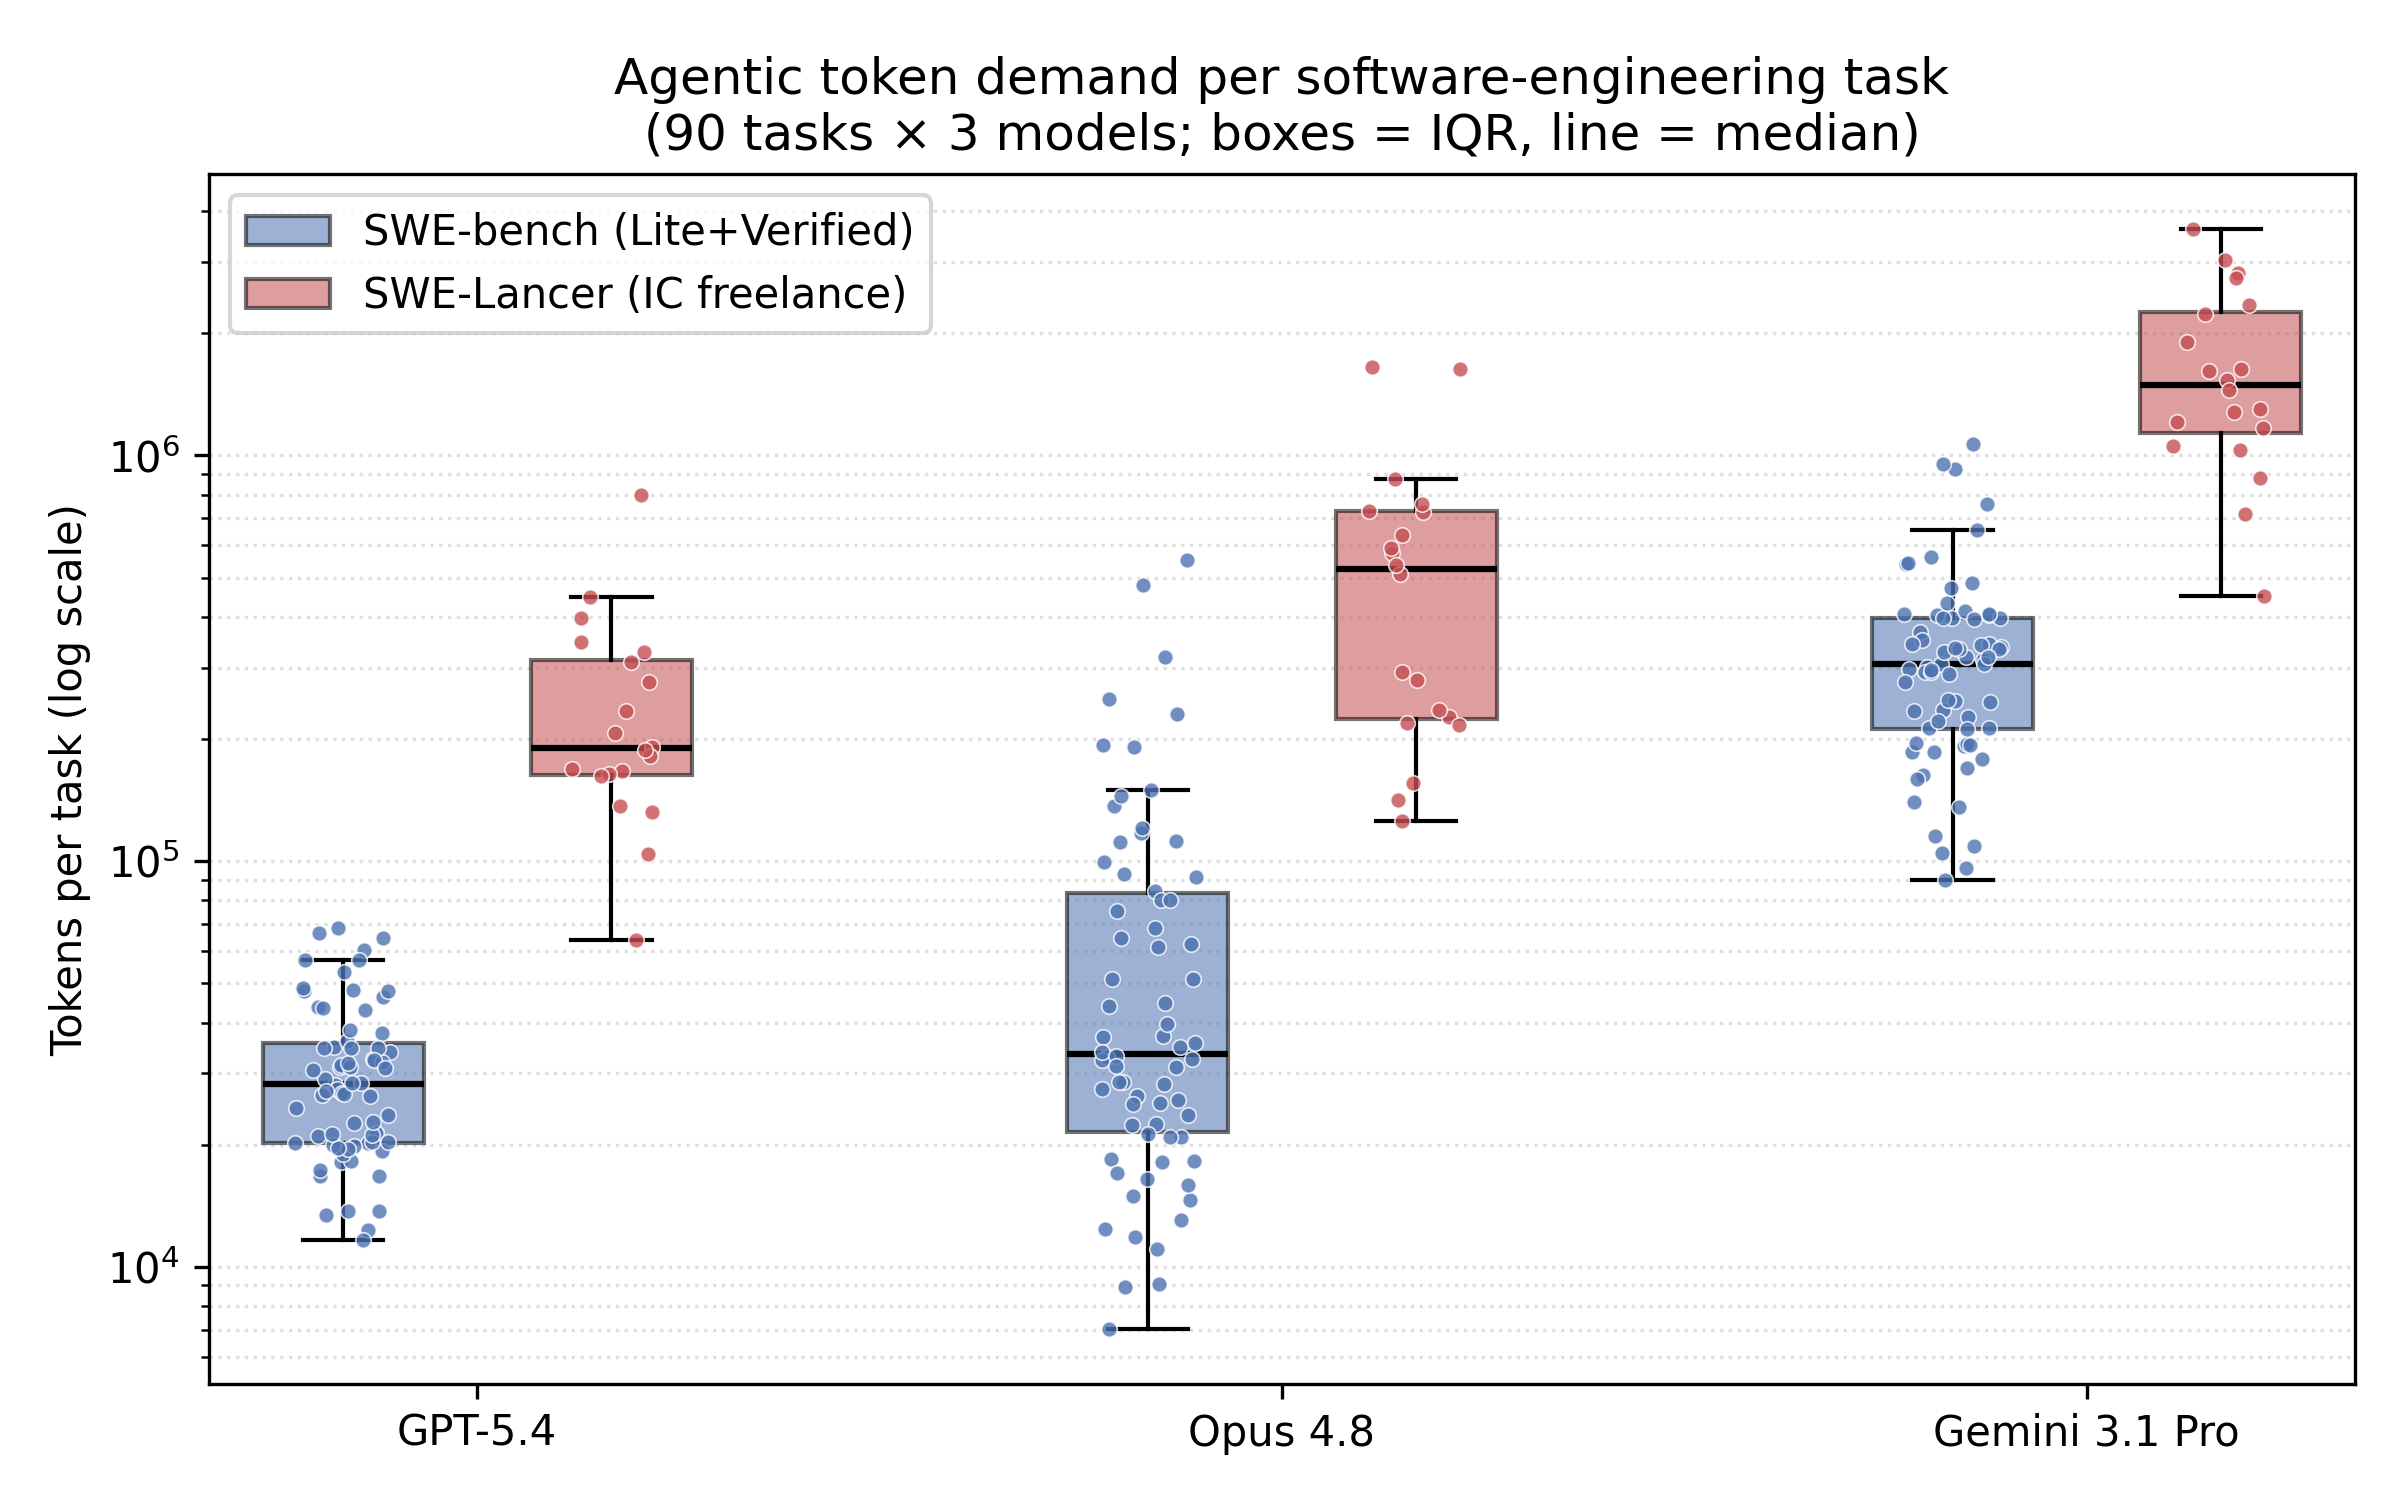
\includegraphics[width=0.5\linewidth]{figures/Fig_2_token_consumption.png}
    \caption{Distribution of cumulative token demand per software-engineering task across three frontier commercial coding models. Each point represents one task execution. Boxes indicate the interquartile range (IQR), the horizontal line denotes the median, and whiskers extend to 1.5$\times$IQR. The y-axis is shown on a logarithmic scale.
    }
    \label{fig:token_distribution}
\end{figure}

As summarized in Table 3, token-demand experiments were conducted on 90 software-engineering tasks using three frontier commercial models, while throughput experiments were performed on four representative open-weight coding models under nine deployment configurations each.

\begin{itemize}
    \item Real-world software engineering consumes one order of magnitude more tokens than SWE-bench.
    \item Model choice changes token demand by approximately one order of magnitude.
    \item The distribution is highly heavy-tailed.
    \item Tool/context processing dominates (>60\%), while generated tokens contribute <1\%.
\end{itemize}

 \begin{equation}
f(x;\mu,\sigma)
=
\frac{1}{x\sigma\sqrt{2\pi}}
\exp\left(
-\frac{(\ln x-\mu)^2}{2\sigma^2}
\right),
\qquad x>0.
\label{eq:token_consumption_dist}
\end{equation}
    



\subsection{Token generation test}

\begin{figure}
    \centering
    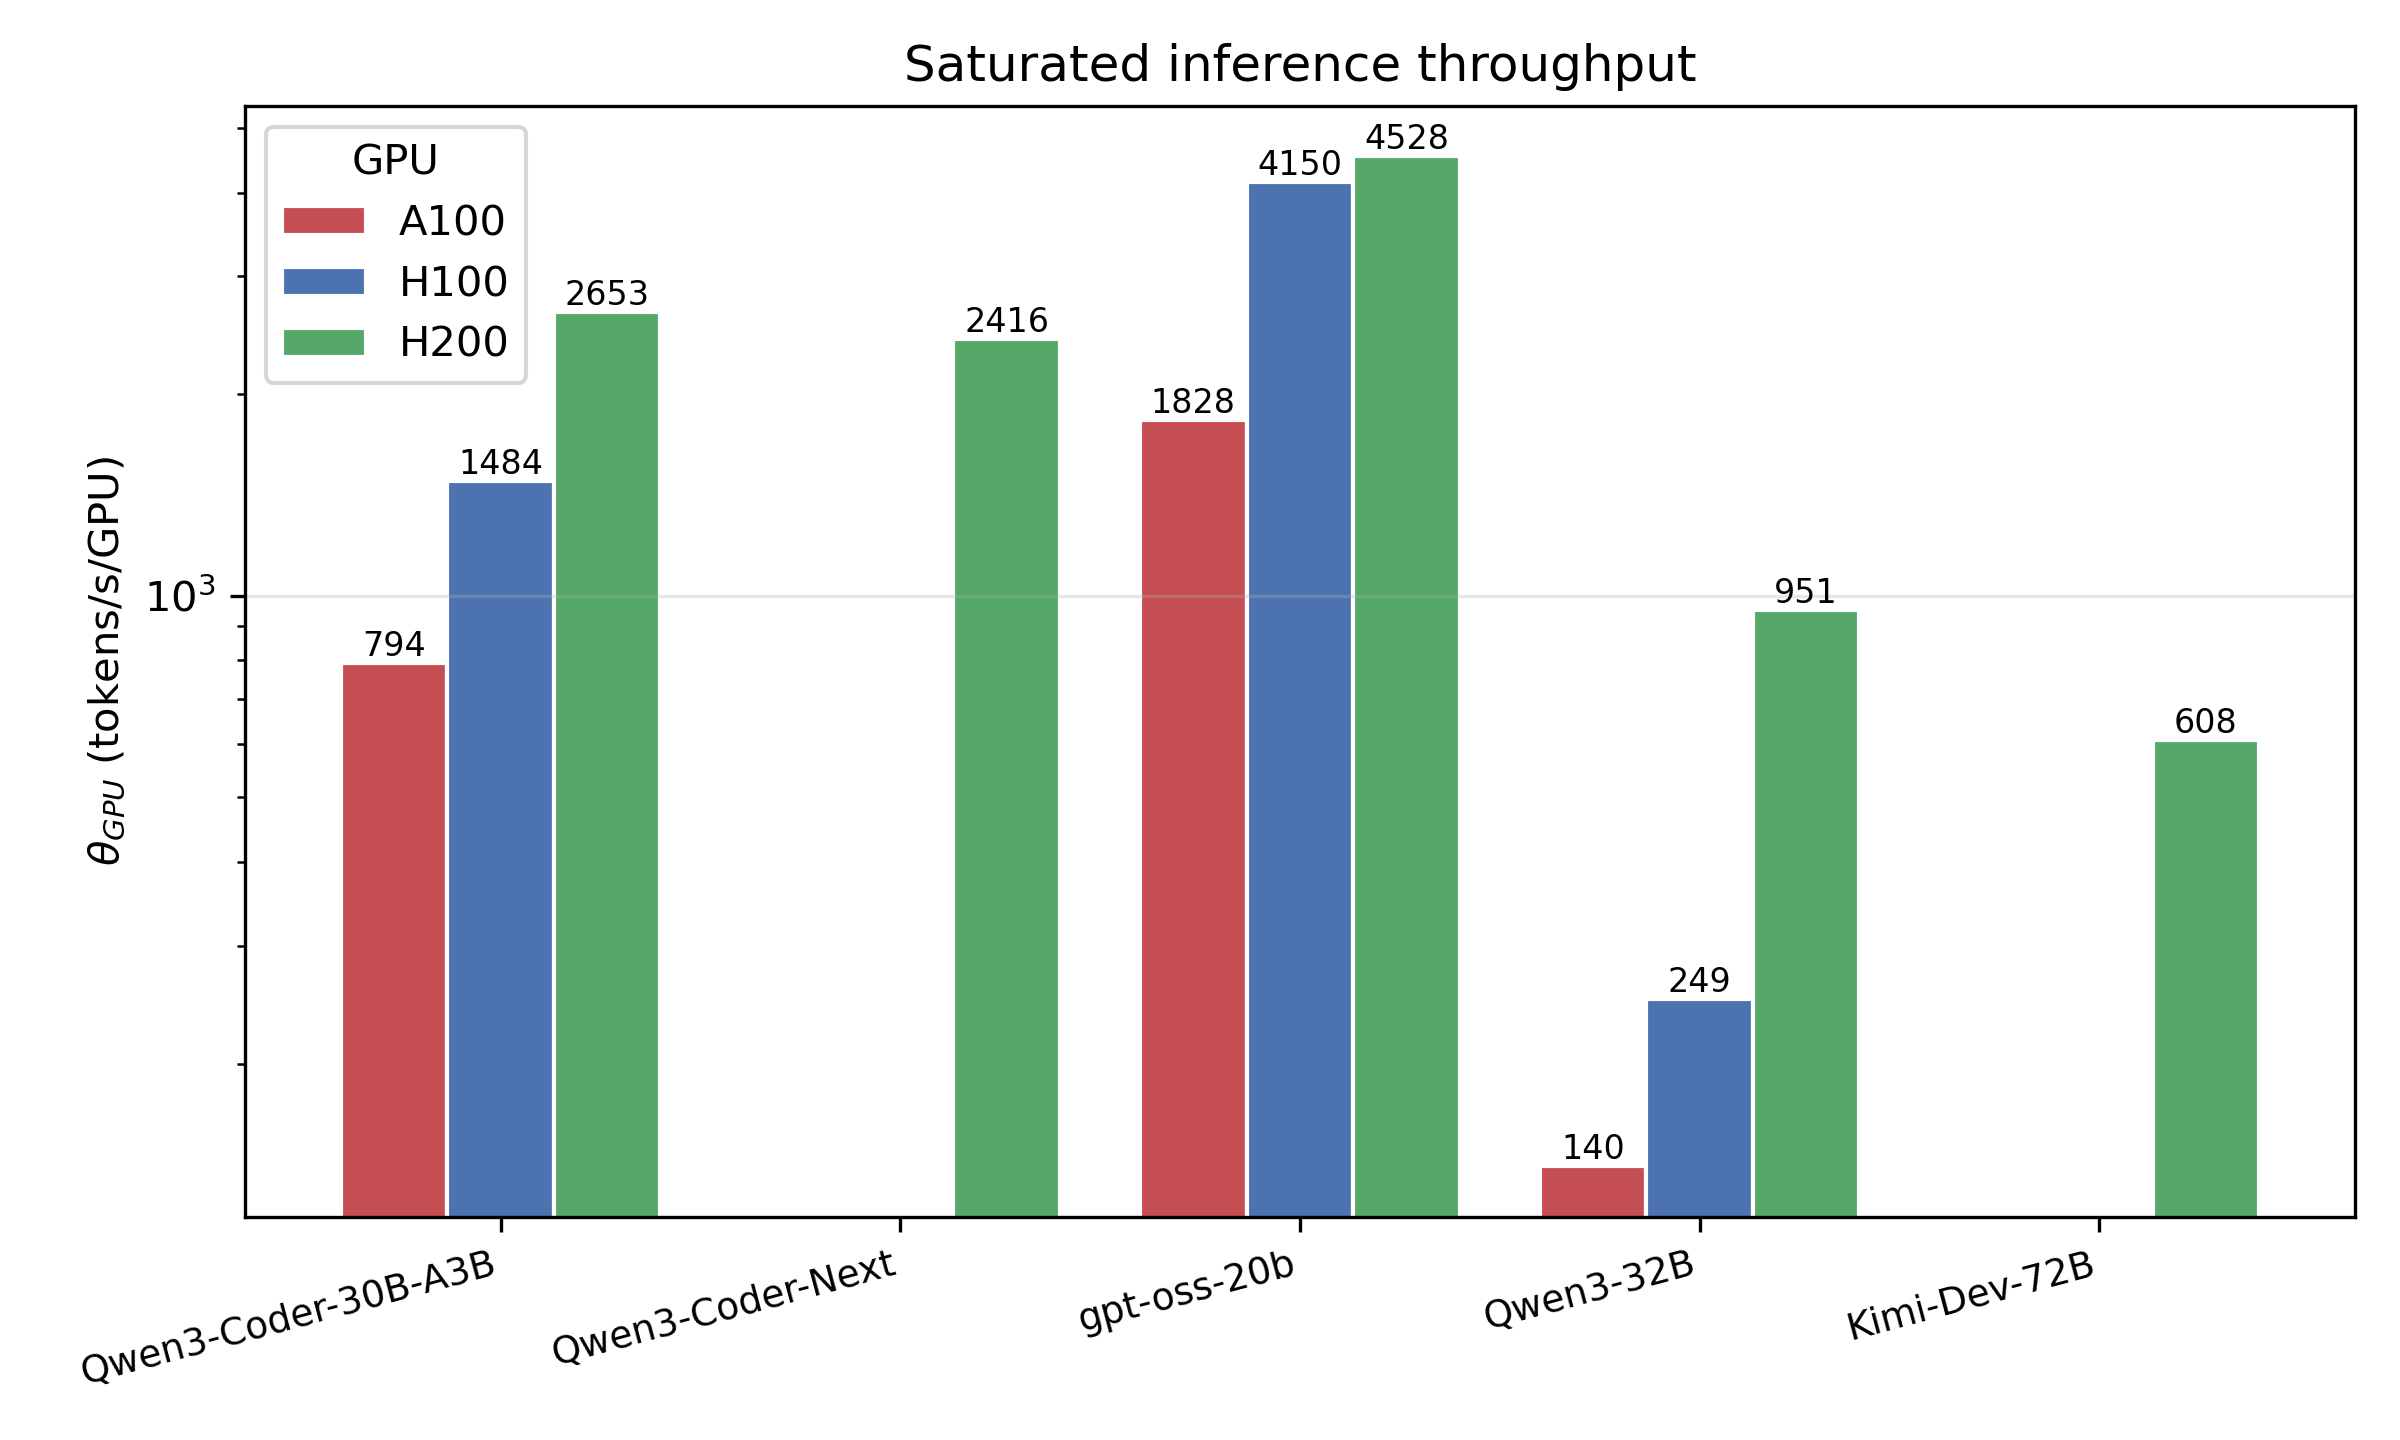
\includegraphics[width=0.5\linewidth]{figures/Fig_3_throughput.png}
    \caption{Inference throughput of representative open-weight coding models on A100, H100, and H200 GPUs. Throughput is reported under saturated serving conditions. MoE models substantially outperform dense models with similar total parameter counts because only a small subset of parameters is activated during inference.}
    \label{fig:inference_throughput}
\end{figure}

\begin{figure}
    \centering
    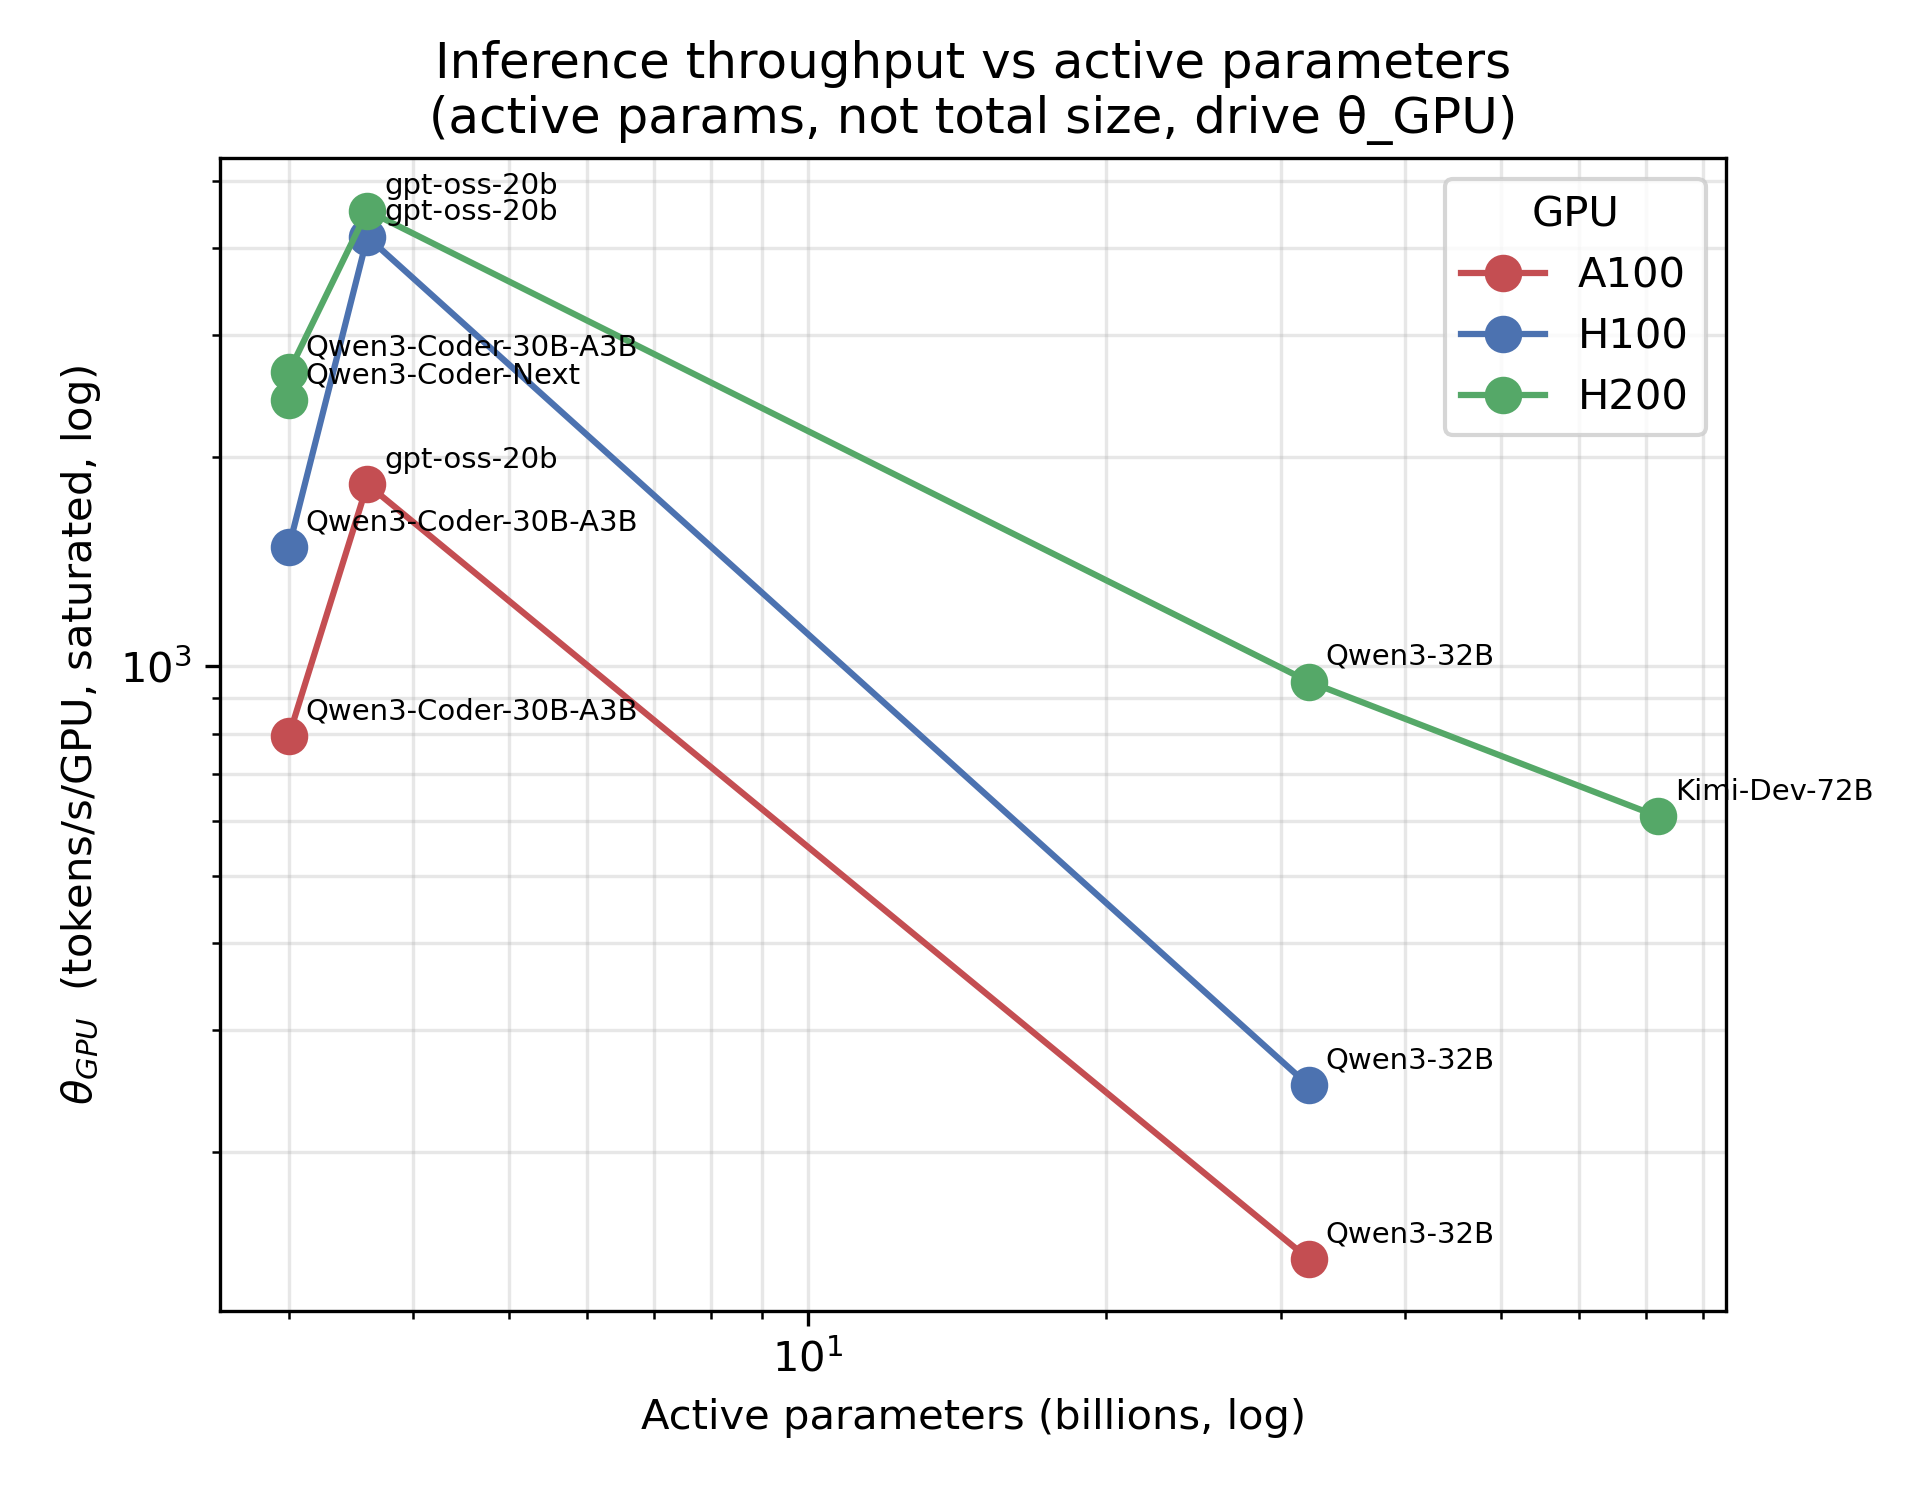
\includegraphics[width=0.5\linewidth]{figures/Fig_4_active_scaling.png}
    \caption{Inference throughput as a function of active model parameters. Active rather than total parameter count explains most of the observed variation in serving throughput.}
    \label{fig:placeholder}
\end{figure}

\begin{figure}
    \centering
    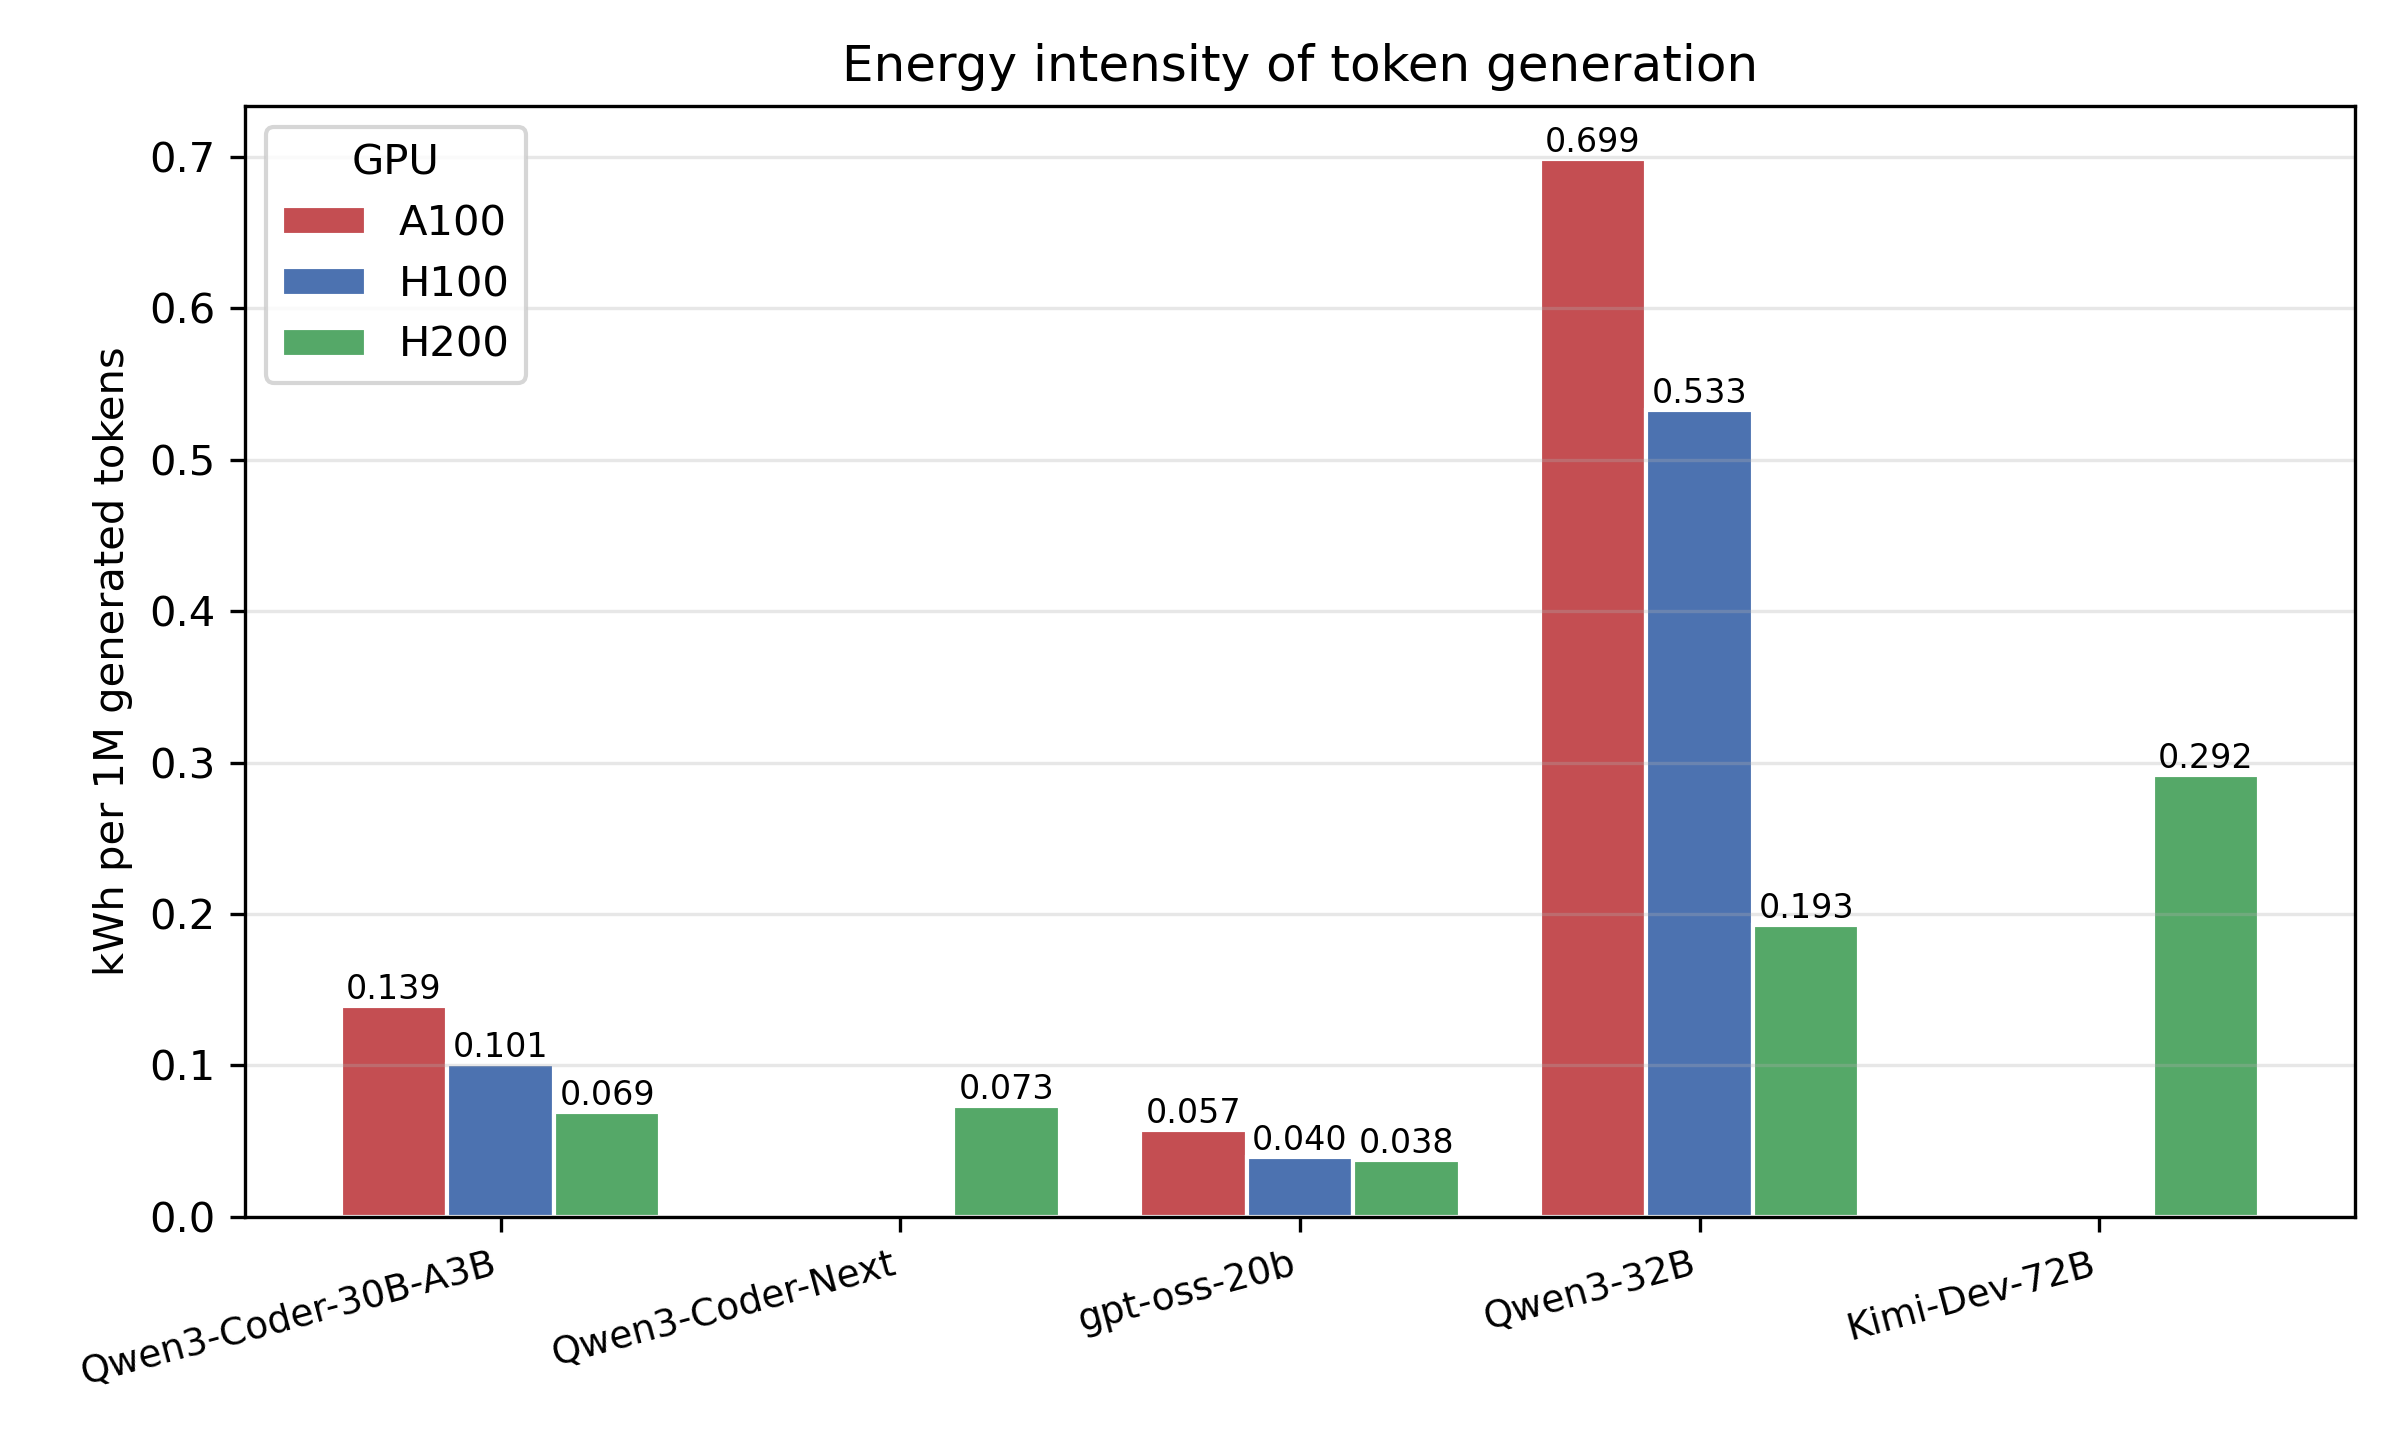
\includegraphics[width=0.5\linewidth]{figures/Fig_5_energy.png}
    \caption{Energy required to generate one million tokens across different models and GPU platforms. Higher throughput directly translates into lower energy intensity, making small-active-parameter MoE models substantially more energy efficient than dense models.}
    \label{fig:placeholder}
\end{figure}


Figure~\ref{fig:throughput}
shows that inference throughput is primarily determined by the number of active parameters rather than total model size.

Across all hardware platforms, MoE models consistently achieve substantially higher throughput and lower energy consumption than dense models with comparable parameter counts.

The advantage of H200 is substantially larger for memory-bound dense models than for compute-bound MoE models, indicating that memory bandwidth becomes the dominant bottleneck as active parameter count increases.

These experimentally measured throughput and energy characteristics provide the infrastructure parameters used in the labor-to-compute model developed in Section~\ref{sec:model}.

The central finding of Experiment 2 is that the number of active parameters, rather than total model size, is the primary determinant of inference throughput. This throughput difference directly translates into differences in energy intensity, establishing the key bridge from token demand to infrastructure cost in the proposed modeling framework.

\subsection{Simulation results}
This section reports the main outputs of the five-layer model. The results focus
on four quantities: engineering labor substitution, token demand, compute
throughput, and energy/economic cost. The purpose is not to forecast a single
future outcome, but to show how software-engineering labor substitution maps
onto AI inference infrastructure under transparent assumptions.

The reconstructed trajectories further reveal that
agentic software engineering is overwhelmingly dominated by
context processing rather than token generation.

Across all models,
generated output accounts for less than 1\%
of total token consumption,
whereas tool observations contribute between
58\% and 86\%.

This finding indicates that the computational bottleneck
of autonomous software engineering lies in repeatedly
processing long execution contexts
rather than decoding generated code.
Consequently,
future infrastructure optimization should primarily target
prefill efficiency,
context caching,
and tool-observation compression,
instead of output-token generation.


% Zitong's Addition.
\subsection{Environmental Externality Results}
\label{subsec:environmental_externality_results}

This section applies the carbon and air-pollution externality framework from Section~2.5 to the scenario matrix reported in Appendix~A.2. The objective is to translate the facility-level electricity requirements implied by AI software-engineering
substitution into greenhouse-gas emissions, monetized climate damages, local air-pollution damages, and total environmental externalities. The power values in the scenario matrix are treated as facility-level central estimates. Therefore, annual
electricity use is computed as

\begin{equation}
E_{\mathrm{annual}} = P_{\mathrm{facility}}\times 8760 .
\end{equation}

Because these power values are already interpreted as facility-level power, PUE is not reapplied in the baseline externality calculation. The PUE values in Table~\ref{tab:externality_parameters_revised} are instead used to interpret upstream facility-power sensitivity when recomputing facility power from IT power.

We then convert annual electricity consumption into greenhouse-gas emissions, monetized climate damages, and monetized air-pollution damages using the environmental parameters summarized in Table~\ref{tab:externality_parameters_revised}. The calculation distinguishes two carbon-accounting concepts. The main results in Table~\ref{tab:externality_results_revised} use location-based average eGRID emission factors, which answer an attributional electricity-accounting question. The marginal
CO$_2$ factors in Table~\ref{tab:externality_parameters_revised} are used separately as an alternative causal-emissions sensitivity, because marginal emissions estimate the generators that respond to incremental AI electricity demand. They should therefore
replace, rather than be added to, the average eGRID CO$_2$e factors.

The analysis reports three location-based environmental cases. The low-emissions case uses the California eGRID subregion (CAMX) and the low social cost of carbon. The central case uses the U.S. average eGRID emission rate and the EPA central social cost of carbon. The high-emissions case uses the Puerto Rico Miscellaneous eGRID subregion (PRMS) and the high social cost of carbon. The high case is not intended to represent a
typical hyperscale siting location. It bounds the externality under a carbon- and pollution-intensive electricity mix. For local air pollution, the screening calculation includes NO$_x$ and SO$_2$ because these pollutants are reported consistently in the eGRID summary table and have electricity-generating-unit benefit-per-ton values in EPA BenMAP. This is a limited-scope screening estimate because it omits primary PM$_{2.5}$, NH$_3$, and VOCs, and it does not replace a site-specific AVERT/COBRA or InMAP analysis.

\begin{table}[htbp]
\centering
\caption{Environmental parameters used in the Section~2.5 externality calculation.
Average CO$_2$e, NO$_x$, and SO$_2$ emission factors are from eGRID 2023 total-output
rates. Air-pollution damage values use EPA BenMAP electricity-generating-unit
benefit-per-ton estimates. EPA BenMAP values are benefits in 2025 but reported in
2016 dollars; the table inflates them to 2025 dollars using CPI-U. Marginal CO$_2$
factors are included as an alternative causal-emissions sensitivity, not as an additive
term to average eGRID CO$_2$e.}
\label{tab:externality_parameters_revised}
\resizebox{\textwidth}{!}{
\begin{tabular}{lcccc}
\toprule
Parameter & Low case & Central case & High case & Source / interpretation \\
\midrule

\multicolumn{5}{l}{\textit{Location-based average-emissions accounting}} \\
\midrule

Average CO$_2$e emission factor (lb/MWh) 
& 429.983 & 770.884 & 1548.530 
& eGRID 2023 CAMX / U.S. average / PRMS \citep{epa_egrid2023_summary} \\

NO$_x$ emission factor (lb/MWh) 
& 0.332 & 0.452 & 3.902 
& eGRID 2023 CAMX / U.S. average / PRMS \citep{epa_egrid2023_summary} \\

SO$_2$ emission factor (lb/MWh) 
& 0.020 & 0.359 & 3.695 
& eGRID 2023 CAMX / U.S. average / PRMS \citep{epa_egrid2023_summary} \\

% \midrule
% \multicolumn{5}{l}{\textit{Alternative marginal-emissions accounting}} \\
% \midrule

% Marginal CO$_2$ factor (lb/kWh) 
% & 0.77 & 1.21 & 2.30 
% & Short-run marginal CO$_2$ range from Graff Zivin et al.; use instead of average CO$_2$e factor \citep{graff_zivin_2014_marginal} \\

% Long-run marginal CO$_2$e factor 
% & \multicolumn{3}{c}{Region-, year-, and scenario-specific} 
% & Implement with NREL Cambium LRMER for long-lived data-center load \citep{nrel_cambium_lrmer2023} \\
\midrule
\multicolumn{5}{l}{\textit{Alternative marginal-emissions accounting}} \\
\midrule

Short-run marginal CO$_2$ factor (lb/kWh) 
& 1.04 & 1.43 & 1.84
& EPA AVERT v4.3 2023 Uniform EE: California / national weighted average / Rocky Mountains; use instead of average eGRID CO$_2$e for near-term incremental load \citep{epa_avert_rates_2024} \\

Long-run marginal CO$_2$ factor (lb/kWh)
& 0.085 & 0.340 & 0.564
& NREL Cambium 2023 levelized LRMER, 2025 start, 20-year evaluation period, 3\% discount rate, Mid-case, end-use load; min / median / max across GEA regions \citep{nrel_cambium_lrmer2023,doe_bto_ghg_metrics_2025} \\

\midrule
\multicolumn{5}{l}{\textit{Damage valuation}} \\
\midrule

Social cost of CO$_2$ (\$/tCO$_2$) 
& 120 & 190 & 340 
& EPA SC-GHG sensitivity cases \citep{epa_scghg2023} \\

NO$_x$ PM$_{2.5}$-related damage (\$/short ton, 2025\$) 
& \multicolumn{3}{c}{10,342} 
& EPA BenMAP EGU value, 2016\$ inflated to 2025\$ \citep{epa_benmap_bpt_2026,bls_cpi_u_annual} \\

NO$_x$ ozone-related damage (\$/short ton, 2025\$) 
& \multicolumn{3}{c}{132,663} 
& EPA BenMAP EGU value, 2016\$ inflated to 2025\$ \citep{epa_benmap_bpt_2026,bls_cpi_u_annual} \\

NO$_x$ total damage used in baseline (\$/short ton, 2025\$) 
& \multicolumn{3}{c}{143,006} 
& PM$_{2.5}$ + ozone benefits for EGU NO$_x$ \citep{epa_benmap_bpt_2026,bls_cpi_u_annual} \\

SO$_2$ damage (\$/short ton, 2025\$) 
& \multicolumn{3}{c}{76,459} 
& EPA BenMAP EGU value, 2016\$ inflated to 2025\$ \citep{epa_benmap_bpt_2026,bls_cpi_u_annual} \\

\midrule
\multicolumn{5}{l}{\textit{Datacenter efficiency}} \\
\midrule

PUE 
& 1.15 & 1.30 & 1.56 
& Efficient AI hyperscale / new-build central / industry-average high case \citep{shehabi_2024_data_center, uptime_2024_survey, uptime_2024_pue} \\

Extreme PUE stress case 
& \multicolumn{3}{c}{1.70} 
& Legacy or inefficient non-hyperscale stress case; not used in baseline AI-hyperscale results \citep{epa_datacenter_report_2007} \\

\bottomrule
\end{tabular}
}
\end{table}

Table~\ref{tab:externality_results_revised} reports the resulting location-based externalities. Because the same central environmental parameters are applied to each scenario, the results scale approximately linearly with facility power. Under the central environmental case, the central agentic scenario consumes 0.964 TWh/yr of electricity and emits approximately 337 ktCO$_2$e/yr. The corresponding monetized climate damage is \$64.0 million/yr. Using EPA BenMAP electricity-generating-unit NO$_x$ and SO$_2$ benefit-per-ton values inflated to 2025 dollars, the screening NO$_x$+SO$_2$ air-pollution damage is \$44.4 million/yr. The total environmental externality is therefore \$108.4 million/yr, or approximately \$15.1 per substituted FTE-year.

The same central agentic scenario spans \$46.2--\$635.1 million/yr across the low-to-high location-based environmental cases. This wide range is not driven by AI workflow uncertainty, which is already embedded in the scenario matrix, but by electricity-sector assumptions, icluding grid carbon intensity, social cost of carbon, NO$_x$ and SO$_2$ emission rates, and the monetized health damages assigned to those pollutants.

\begin{table}[htbp]
\centering
\caption{Carbon and air-pollution externality results using the revised Table~3 parameters. Central values use U.S. average eGRID 2023 emission rates, EPA central SCC of \$190/tCO$_2$, and EPA BenMAP EGU NO$_x$+SO$_2$ benefit-per-ton values inflated to 2025 dollars. Bracketed ranges combine the low-emissions CAMX/low-SCC case and the high-emissions PRMS/high-SCC case. Air-pollution damages include NO$_x$ and SO$_2$ only and should be interpreted as a limited-scope screening estimate.}
\label{tab:externality_results_revised}
\resizebox{\textwidth}{!}{
\begin{tabular}{lrrrrrrrr}
\toprule
Scenario
& Power
& Electricity
& CO$_2$e
& Climate damage
& Air damage
& Externality
& Externality range
& Externality / FTE \\
& (MW)
& (TWh/yr)
& (kt/yr)
& (\$M/yr)
& (\$M/yr)
& (\$M/yr)
& (\$M/yr)
& (\$/FTE-yr) \\
\midrule
Conservative agentic
& 36.8 & 0.322 & 113 & 21.4 & 14.8 & 36.3 & [15.4, 212.5] & 15.1 \\

Central agentic
& 110.0 & 0.964 & 337 & 64.0 & 44.4 & 108.4 & [46.2, 635.1] & 15.1 \\

Aggressive agentic
& 293.0 & 2.567 & 897 & 170.5 & 118.2 & 288.7 & [123.0, 1691.6] & 15.0 \\

Conservative copilot
& 12.3 & 0.108 & 38 & 7.2 & 5.0 & 12.1 & [5.2, 71.0] & 5.0 \\

Central copilot
& 36.7 & 0.321 & 112 & 21.4 & 14.8 & 36.2 & [15.4, 211.9] & 5.0 \\

Aggressive copilot
& 97.9 & 0.858 & 300 & 57.0 & 39.5 & 96.5 & [41.1, 565.2] & 5.0 \\
\bottomrule
\end{tabular}
}
\end{table}

Several results are worth emphasizing. First, environmental externalities are small relative to the economic value of substituted software-engineering labor, but they are not small relative to private electricity cost. In the central agentic case, the total environmental externality is \$108.4 million/yr. This corresponds to roughly \$112/MWh of facility electricity consumption, composed of about \$66/MWh in climate
damages and \$46/MWh in screening NO$_x$+SO$_2$ health damages. Thus, under the central U.S.-average case, environmental externalities are of the same order as, and may exceed, the private electricity bill depending on the assumed electricity price.

Second, climate damages are the larger component in the central U.S.-average case, but air-pollution damages are not a residual term. For the central agentic scenario, air-pollution damages account for \$44.4 million/yr, or approximately 41\% of the total environmental externality. This reflects the relatively high EPA BenMAP electricity-generating-unit benefit-per-ton value for NO$_x$, especially after including both PM$_{2.5}$-related and ozone-related health damages. In the high-emissions PRMS case, local air-pollution damages can become even more important because NO$_x$ and SO$_2$ emission rates rise much faster than the average CO$_2$e factor.

Third, the per-FTE externality is approximately constant within each operating mode because the scenario matrix scales facility power approximately proportionally with substituted FTEs. Agentic scenarios produce about \$15/FTE-yr of environmental externality under the central environmental case, whereas copilot scenarios produce about \$5/FTE-yr. This does not mean that copilot workloads are intrinsically cleaner on a per-token basis. It reflects the facility-power assumptions embedded in the scenario matrix. The environmental layer therefore inherits the upstream modeling assumptions about tokens, throughput, utilization, and facility power.

To identify the dominant environmental uncertainty sources, we perform a one-way sensitivity analysis around the central agentic scenario. Table~\ref{tab:externality_sensitivity_revised} varies one parameter group at a time while holding all other parameters fixed at central values. The baseline total environmental externality is \$108.4 million/yr as shown in Table~\ref{tab:externality_results_revised}. 

\begin{table}[htbp]
\centering
\caption{One-way sensitivity analysis for the central agentic scenario using the revised Table~\ref{tab:externality_parameters_revised} parameters. The baseline total environmental externality is \$108.4 million/yr, consisting of \$64.0 million/yr in climate damages and \$44.4 million/yr in screening NO$_x$+SO$_2$ air-pollution damages. Each row varies one parameter group while holding all other parameters fixed at central values. The marginal CO$_2$ row is an alternative carbon-accounting case that replaces the location-based average CO$_2$e factor rather than adding to it.}
\label{tab:externality_sensitivity_revised}
\resizebox{\textwidth}{!}{
\begin{tabular}{lccc}
\toprule
Parameter varied 
& Low-result externality 
& High-result externality 
& Half-width of sensitivity range \\
& (\$M/yr) & (\$M/yr) & (\$M/yr) \\
\midrule

NO$_x$/SO$_2$ emission rates 
& 87.6 & 469.0 & 190.7 \\

% Alternative marginal CO$_2$ factor 
% & 108.3 & 235.4 & 63.5 \\
Alternative short-run marginal CO$_2$ factor & 130.5 & 197.2 & 33.3 \\

Alternative long-run marginal CO$_2$ factor & 51.5 & 91.2 & 19.9 \\

Average grid CO$_2$e factor 
& 80.1 & 173.0 & 46.4 \\

Social cost of carbon 
& 84.8 & 158.9 & 37.1 \\

Air-pollution damage factors 
& 86.2 & 152.8 & 33.3 \\

Facility power / PUE scaling 
& 95.9 & 130.1 & 17.1 \\

\bottomrule
\end{tabular}
}
\end{table}

The sensitivity analysis changes the interpretation of the environmental results. With the revised EPA BenMAP air-pollution damage factors, the largest one-way sensitivity is
the NO$_x$/SO$_2$ emissions-rate case, not the average grid CO$_2$e factor. Varying the NO$_x$ and SO$_2$ emission rates from the CAMX case to the PRMS case changes the central agentic externality from \$87.6 million/yr to \$469.0 million/yr. The large upper-end result occurs because the PRMS case combines high NO$_x$ and SO$_2$ emission rates with high monetized health damages per ton. This finding shows that AI datacenter siting is not only a carbon problem, but also a local air-quality problem.

% The marginal CO$_2$ row should be interpreted separately. It replaces the average eGRID CO$_2$e factor with short-run marginal CO$_2$ factors and then adds the central NO$_x$+SO$_2$ air-damage estimate for comparability. The low marginal CO$_2$ factor of 0.77 lb/kWh is almost identical to the U.S. average eGRID factor of 770.884 lb/MWh, which is why the low-result marginal externality (\$108.3 million/yr) is nearly identical
% to the location-based baseline (\$108.4 million/yr). The high marginal CO$_2$ factor, however, increases the total externality to \$235.4 million/yr. This illustrates why average-emissions accounting can either understate or overstate causal emissions, depending on the marginal generator mix.

The location-based accounting above should be complemented with marginal-emissions checks. Location-based eGRID factors answer an attributional Scope~2 accounting question, whereas marginal emissions better approximate the causal effect of adding new AI load to the grid. We update the short-run marginal-emissions sensitivity using EPA AVERT v4.3 2023 Uniform EE rates, interpreted as the avoided-emissions counterpart of a flat 24/7
incremental datacenter load. Under this short-run dispatch interpretation, the central agentic scenario produces climate-only marginal damages of \$86.1--\$152.8 million/yr at an SCC of \$190/tCO$_2$. Adding central NO$_x$+SO$_2$ screening damages gives a total short-run marginal externality range of \$130.5--\$197.2 million/yr.

For long-lived datacenter investments, however, short-run marginal rates are incomplete because the load may also affect generation investment, retirement, and transmission planning. We therefore also report NREL Cambium 2023 long-run marginal emission rates as a separate sensitivity. Using the levelized Cambium LRMER range gives substantially lower climate-only damages, because the modeled long-run grid partially decarbonizes and adapts to demand changes. These marginal-emissions calculations should not be added to the location-based eGRID CO$_2$e estimate. They are alternative causal-emissions pathways. A final implementation should use region- and hour-specific AVERT, Cambium, or nodal locational marginal emissions rather than a national scalar.

The average grid CO$_2$e factor and the social cost of carbon remain important, but their one-way ranges are smaller than the NO$_x$/SO$_2$ emission-rate range in this screening analysis. Varying the average CO$_2$e factor changes the total externality from \$80.1 million/yr to \$173.0 million/yr, while varying the social cost of carbon changes it from \$84.8 million/yr to \$158.9 million/yr. In contrast, varying air-pollution damage factors alone changes the result from \$86.2 million/yr to \$152.8 million/yr. These comparisons indicate that the physical location and emissions profile of the electricity supply are at least as important as the valuation parameters used to monetize damages.

The facility-power/PUE row is the smallest sensitivity in Table~\ref{tab:externality_sensitivity_revised}, but it should be interpreted carefully. Because Table~\ref{tab:externality_results_revised} uses scenario-matrix power as facility-level power, PUE is not applied a second time in the baseline. The PUE sensitivity instead represents the proportional effect of recomputing facility power from IT power using the PUE range in
Table~\ref{tab:externality_parameters_revised}. Under this interpretation, facility-power scaling changes the central agentic externality from \$95.9 million/yr to \$130.1 million/yr.

Overall, the environmental externality analysis supports three conclusions. First, environmental damages are modest on a per-substituted-FTE basis, but they are material relative to the private electricity bill. Second, carbon damages alone are insufficient for evaluating AI datacenter siting because NO$_x$ and SO$_2$ health damages can dominate the uncertainty range in pollution-intensive regions. Third, location-based accounting
should be complemented with marginal-emissions analysis for incremental AI load. In a final implementation, hourly inference-load profiles should be combined with AVERT short-run marginal emissions or NREL Cambium long-run marginal emissions, depending on whether the analysis is framed as a near-term dispatch problem or a long-lived datacenter investment problem.

% End of Zitong's addition.







% ─────────────────────────────────────────────────────────────────────────────
\subsection{Discussion}
\label{sec:discussion}

6.1 Why Energy Cost Appears Small Relative to Labor Value
    6.2 Infrastructure Implications
    6.3 Limits of Agentic Software Engineering
    6.4 Policy and Energy-System Implications

\subsubsection{Assumptions and Limitations}
% \label{sec:assumptions}

The token-consumption experiments are conducted using
frontier commercial models,
whereas throughput measurements are obtained using
representative open-weight models.

This design reflects the practical separation between
capability estimation and infrastructure characterization.
Commercial APIs provide the most capable publicly available
software-engineering agents but do not expose
their underlying hardware or serving configurations.
Conversely,
open-weight models can be deployed on controlled GPU
hardware, enabling direct measurement of throughput,
utilization, and power consumption.

Accordingly,
the first experiment estimates the inference workload
required to solve software-engineering tasks,
whereas the second experiment estimates the physical
resources required to execute a given inference workload.

% The model developed in this paper is a scenario framework rather than a
% point forecast. Its purpose is to make the chain from software-engineering labor
% substitution to token demand, compute throughput, energy use, cost, and market
% size explicit and auditable. Because several parameters are uncertain or rapidly
% changing, the paper separates locked modeling assumptions from values that
% require pre-publication verification.

% \subsection{Locked Modeling Assumptions}
% \label{sec:locked-assumptions}

% During the research phase, several parameters were found to have either
% conflicting estimates across sources or no single authoritative empirical value.
% For each such parameter, the model selects a working value for the central case
% and reports a plausible range for sensitivity analysis. These assumptions should
% not be interpreted as claims about the true future value of the parameter; they
% are modeling inputs used to make the scenario calculations internally
% consistent.

% \begin{table}[htbp]
% \centering
% \caption{Locked Modeling Assumptions: Conflicts and Decisions}
% \label{tab:locked-assumptions}
% \small
% \begin{tabular}{@{}p{3.4cm}p{2.5cm}p{2.6cm}p{4.8cm}@{}}
% \hline
% \textbf{Parameter} & \textbf{Central Value} & \textbf{Sensitivity Range} & \textbf{Rationale} \\
% \hline
% Global software engineering FTEs
% & 24 million
% & 20--29 million
% & Uses a midpoint between major global developer-population estimates. The model treats this as a rounded FTE-equivalent workforce anchor rather than a precise headcount. \\

% Effective substitution rate, $s$
% & 30\%
% & 10\%--80\%
% & The central case represents AI agents becoming a normal supervised production workforce. The 10\% case is conservative; 50--60\% is aggressive; 80\% is retained only as an extreme stress scenario. \\

% Tokens per replaced FTE-day, $T_{\mathrm{FTE}}$
% & 4 million
% & $10^{5}$--$10^{7+}$
% & The central case represents agentic software production with planning, coding, testing, debugging, and retries. Lower values correspond to Copilot-style assistance; higher values correspond to frontier reasoning agents. \\

% H100 inference power draw, $P_{\mathrm{GPU}}$
% & 700 W/GPU
% & 700--1{,}000+ W/GPU-equivalent
% & The central case uses the H100 SXM TDP as a physical power anchor. Higher effective values may arise when accounting for memory, networking, server-level overhead, or less efficient utilization. \\

% GPU utilization factor, $U$
% & Scenario-dependent
% & 40\%--80\%
% & Installed GPU requirements depend on realized utilization, batching efficiency, workload variability, scheduling, memory constraints, and queueing. The model reports utilization explicitly rather than assuming peak theoretical throughput. \\

% Data-center PUE
% & 1.56
% & 1.1--1.8
% & A broad industry-average PUE is used for the central case. Hyperscale frontier facilities may operate closer to 1.1--1.3, while older or less optimized facilities may be higher. \\

% Electricity price, $C_{\mathrm{MWh}}$
% & \$60/MWh
% & \$20--\$120/MWh
% & The central case uses a blended electricity-price assumption. Actual prices vary substantially by geography, contract structure, power source, grid congestion, and duration of procurement. \\

% Data-center construction cost
% & \$15M/MW
% & \$10--\$25M/MW
% & The central case represents an AI-oriented data-center capacity cost between conventional hyperscale and highly constrained liquid-cooled AI facilities. \\

% Model-tier deployment
% & Frontier agentic model
% & Copilot, specialized coding model, frontier API, enterprise-hosted, local/open model
% & The central scenario assumes a capable frontier or near-frontier coding model. Sensitivity cases allow lower-cost specialized or self-hosted models with different capability ceilings. \\
% \hline
% \end{tabular}
% \end{table}

% The most important locked assumptions are $s$ and $T_{\mathrm{FTE}}$. These two
% parameters jointly determine aggregate token demand:

% \begin{equation}
%     D = N_{\mathrm{eng}} \cdot s \cdot T_{\mathrm{FTE}} .
% \end{equation}

% A change in either the substitution rate or the tokens required per replaced
% FTE-day scales total token demand approximately linearly. By contrast,
% improvements in GPU throughput, utilization, and PUE affect the translation from
% token demand into infrastructure and electricity requirements.

% \subsection{Pre-Publication Verification Requirements}
% \label{sec:verification-requirements}

% Several claims used in the draft are appropriate for exploratory modeling but
% should be verified against primary or directly accessible sources before
% publication. Table~\ref{tab:verification} lists the most important verification
% items.

% \begin{table}[htbp]
% \centering
% \caption{Pre-Publication Verification Checklist}
% \label{tab:verification}
% \small
% \begin{tabular}{@{}p{4.2cm}p{3.2cm}p{5.2cm}@{}}
% \hline
% \textbf{Claim or Parameter} & \textbf{Current Status} & \textbf{Verification Action} \\
% \hline
% Agentic coding token consumption, including million-token task ranges and high run-to-run variance
% & Based on recent arXiv evidence; not yet a mature empirical literature
% & Retrieve the full paper, check the experimental setup, models, task distribution, and whether the reported range generalizes beyond the benchmark setting. \\

% Share of work hours technically automatable
% & Secondary automation estimates vary by methodology
% & Use the original McKinsey or comparable labor-automation report directly. Avoid treating a single percentage as a precise software-engineering replacement ceiling. \\

% Global software developer or software-engineering FTE count
% & Estimates differ by definition: professional developers, software developers, ICT workers, or broader engineering occupations
% & State the chosen definition explicitly. Use multiple sources to triangulate and report a sensitivity range rather than relying on a single global count. \\

% GitHub Copilot productivity and adoption metrics
% & Productivity gains and user counts are context-dependent
% & Distinguish controlled-experiment productivity estimates from adoption statistics. Avoid applying a single productivity gain to all engineering work. \\

% Frontier-model API prices
% & Prices change frequently
% & Record the retrieval date and model name. Use API prices as time-stamped scenario inputs, not stable long-run costs. \\

% H100 and B200 throughput assumptions
% & Benchmark-dependent
% & Report model size, precision, batch size, latency constraint, and benchmark source. Treat B200 throughput as an efficiency scenario, not a universal constant. \\

% Data-center construction cost per MW
% & Highly location- and design-dependent
% & Separate conventional hyperscale, AI-optimized, and power-constrained facilities. Triangulate with industry reports and company disclosures. \\

% Large-load, PPA, and nuclear restart deal terms
% & Often reported through company releases and media coverage
% & Use primary company announcements, SEC filings, or contract documents where available. Treat analyst-estimated PPA prices as secondary evidence. \\

% OpenAI global token volume or total daily inference volume
% & No reliable primary source identified
% & Remove from the paper unless a primary or highly credible source is found. Do not use unsourced global token-volume claims as model inputs. \\
% \hline
% \end{tabular}
% \end{table}

% \subsection{Model Limitations}
% \label{sec:model-limitations}

% The model intentionally abstracts from several mechanisms that could materially
% change real-world outcomes. These limitations do not invalidate the framework,
% but they define the boundaries of what the current model can claim.

% \begin{enumerate}
%     \item \textbf{Task substitution is not the same as headcount replacement.}
%     The model uses an effective FTE substitution rate, $s$, to convert
%     task-level automation into labor-equivalent units. In practice, firms may
%     use AI to increase output, reduce hiring growth, shorten development
%     cycles, improve quality, or reallocate engineers rather than directly
%     eliminating positions.

%     \item \textbf{Token demand is highly uncertain.}
%     The number of tokens required per replaced FTE-day depends on task
%     complexity, agent design, model choice, context length, retry rate, tool
%     use, codebase size, and the amount of human supervision. A single central
%     value such as 4 million tokens per FTE-day should be interpreted as a
%     scenario assumption, not a measured universal constant.

%     \item \textbf{The model does not fully capture model-efficiency
%     improvements.}
%     Hardware and model efficiency are improving rapidly. Next-generation
%     accelerators, lower-precision inference, speculative decoding, model
%     distillation, mixture-of-experts architectures, caching, and better agent
%     orchestration could reduce the compute and energy required per useful unit
%     of engineering output.

%     \item \textbf{The model uses simplified workload composition.}
%     The central case treats software-engineering inference as if it can be
%     represented by a small number of token-intensity regimes. In reality,
%     engineering work mixes simple autocomplete, chat-based assistance,
%     repository-level retrieval, long-context reasoning, test generation,
%     debugging, code review, and multi-agent workflows. Many routine tasks may be
%     handled by smaller or specialized models at substantially lower cost.

%     \item \textbf{GPU throughput is benchmark-dependent.}
%     Tokens per second per GPU depends on model size, precision, quantization,
%     memory bandwidth, batch size, sequence length, latency target, serving
%     stack, and utilization. Therefore, hardware results should be read as
%     scenario outputs under specified throughput assumptions rather than as
%     universal GPU requirements.

%     \item \textbf{Electricity cost is not total inference cost.}
%     The physical energy cost of inference is only one component of AI service
%     cost. Full cost also includes GPU depreciation, data-center construction,
%     networking, storage, memory, cooling systems, maintenance, reliability
%     engineering, reserved capacity, software infrastructure, and provider
%     margin. API prices bundle these costs and may differ substantially from
%     self-hosted marginal energy cost.

%     \item \textbf{Geography is simplified.}
%     The model uses a blended electricity price and broad PUE assumptions. Actual
%     data-center economics vary by location, climate, grid congestion, access to
%     firm power, transmission availability, tax incentives, water constraints,
%     land availability, and interconnection timelines.

%     \item \textbf{Institutional adoption friction is not fully modeled.}
%     Even if AI agents become technically capable, adoption may be slowed by
%     procurement cycles, security review, data-governance requirements,
%     intellectual-property concerns, compliance rules, legal liability for
%     AI-generated code, developer trust, and the cost of integrating agents into
%     existing engineering workflows.

%     \item \textbf{Quality, reliability, and verification costs are excluded.}
%     The model counts the cost of generating tokens but does not fully model the
%     cost of validating AI-generated code, repairing subtle bugs, maintaining
%     software over time, handling security vulnerabilities, or assigning human
%     accountability for production failures.

%     \item \textbf{The model does not endogenize Jevons effects.}
%     The central framing asks how much compute and energy would be required to
%     substitute for a given share of existing software-engineering labor.
%     However, cheaper software production may increase total demand for software,
%     leading to more projects, more code, more maintenance, and potentially
%     higher total engineering activity rather than lower total labor demand.

%     \item \textbf{Training and fine-tuning costs are excluded from the main
%     inference model.}
%     The paper focuses on inference required to perform software-engineering
%     work. Training, post-training, fine-tuning, reinforcement learning, data
%     collection, and evaluation workloads may be important for frontier-model
%     providers but are outside the core labor-substitution calculation.

%     \item \textbf{Market sizing is not an investment recommendation.}
%     The market-sizing section estimates potential labor value and infrastructure
%     demand under modeled scenarios. It does not forecast security returns,
%     company-level revenue, valuation multiples, or investment performance.
% \end{enumerate}

% Taken together, these limitations imply that the model should be interpreted as
% a structured sensitivity analysis. Its main contribution is not to predict a
% single future electricity load or market size, but to clarify which parameters
% matter most and how software labor substitution translates into physical
% infrastructure requirements.


We do not claim to know the exact future substitution rate of AI software engineers. Instead, we ask: conditional on a given level of FTE-equivalent substitution, what physical infrastructure is implied, and how uncertain is that estimate?

The largest uncertainties are not electricity price or PUE, but token intensity, retry behavior, effective throughput, and realized substitution. Therefore, the energy implications of AI labor substitution depend more on AI workflow design and model-serving efficiency than on marginal power cost.


% ─────────────────────────────────────────────────────────────────────────────
\section{Conclusion}
\label{sec:conclusion}



% ─────────────────────────────────────────────────────────────────────────────
\section*{Acknowledgments}

The authors thank [TBD] for helpful discussions and feedback on earlier drafts. [Funding
acknowledgment TBD.] All errors remain the authors' own.

% ─────────────────────────────────────────────────────────────────────────────
\bibliographystyle{abbrvnat}
\bibliography{paper}

% ─────────────────────────────────────────────────────────────────────────────
\appendix

\section{Sanity Check: Commercial and Open-Weight Token Demand}
\label{app:sanity}

Experiment~1 estimates token demand using frontier commercial models,
whereas Experiment~2 measures inference throughput using representative
open-weight models. To assess whether these two experimental components
can be reasonably combined, we perform an additional sanity check by
measuring token consumption using an open-weight coding model under the
same agent scaffold.

Specifically, Qwen3-Coder-30B-A3B was deployed using the same vLLM
serving configuration as Experiment~2 and executed through the identical
mini-SWE-agent framework used in Experiment~1. The evaluation was
performed on the same ten SWE-bench Lite tasks previously solved by the
commercial models.

Figure~\ref{fig:appendix_token_parity} compares the total token
consumption of the four models on each task. Although the open-weight
model consistently consumes more tokens than GPT-5.4 and Claude Opus~4.8,
its token demand remains within the same order of magnitude as Gemini~3.1
Pro. Median token consumption is 445k tokens per task for
Qwen3-Coder-30B-A3B, compared with 363k for Gemini~3.1 Pro, 36k for
Claude Opus~4.8, and 32k for GPT-5.4.

The larger token budget of the open-weight model is primarily explained
by more frequent tool-format retries and repeated context replay,
reflecting differences in model capability rather than differences in
task complexity or measurement methodology. Despite requiring more
inference, the open model successfully completed 8 of the 10 benchmark
tasks, demonstrating that it operates within the same agentic software
engineering regime.

Overall, this experiment indicates that token demand is predominantly a
property of the software-engineering task and the agent execution
workflow. While absolute token consumption varies across model families,
commercial and open-weight models exhibit comparable inference workloads
at the order-of-magnitude level, supporting the use of commercial models
to characterize task demand and open-weight models to characterize
hardware throughput in the main study.

\begin{figure}
    \centering
    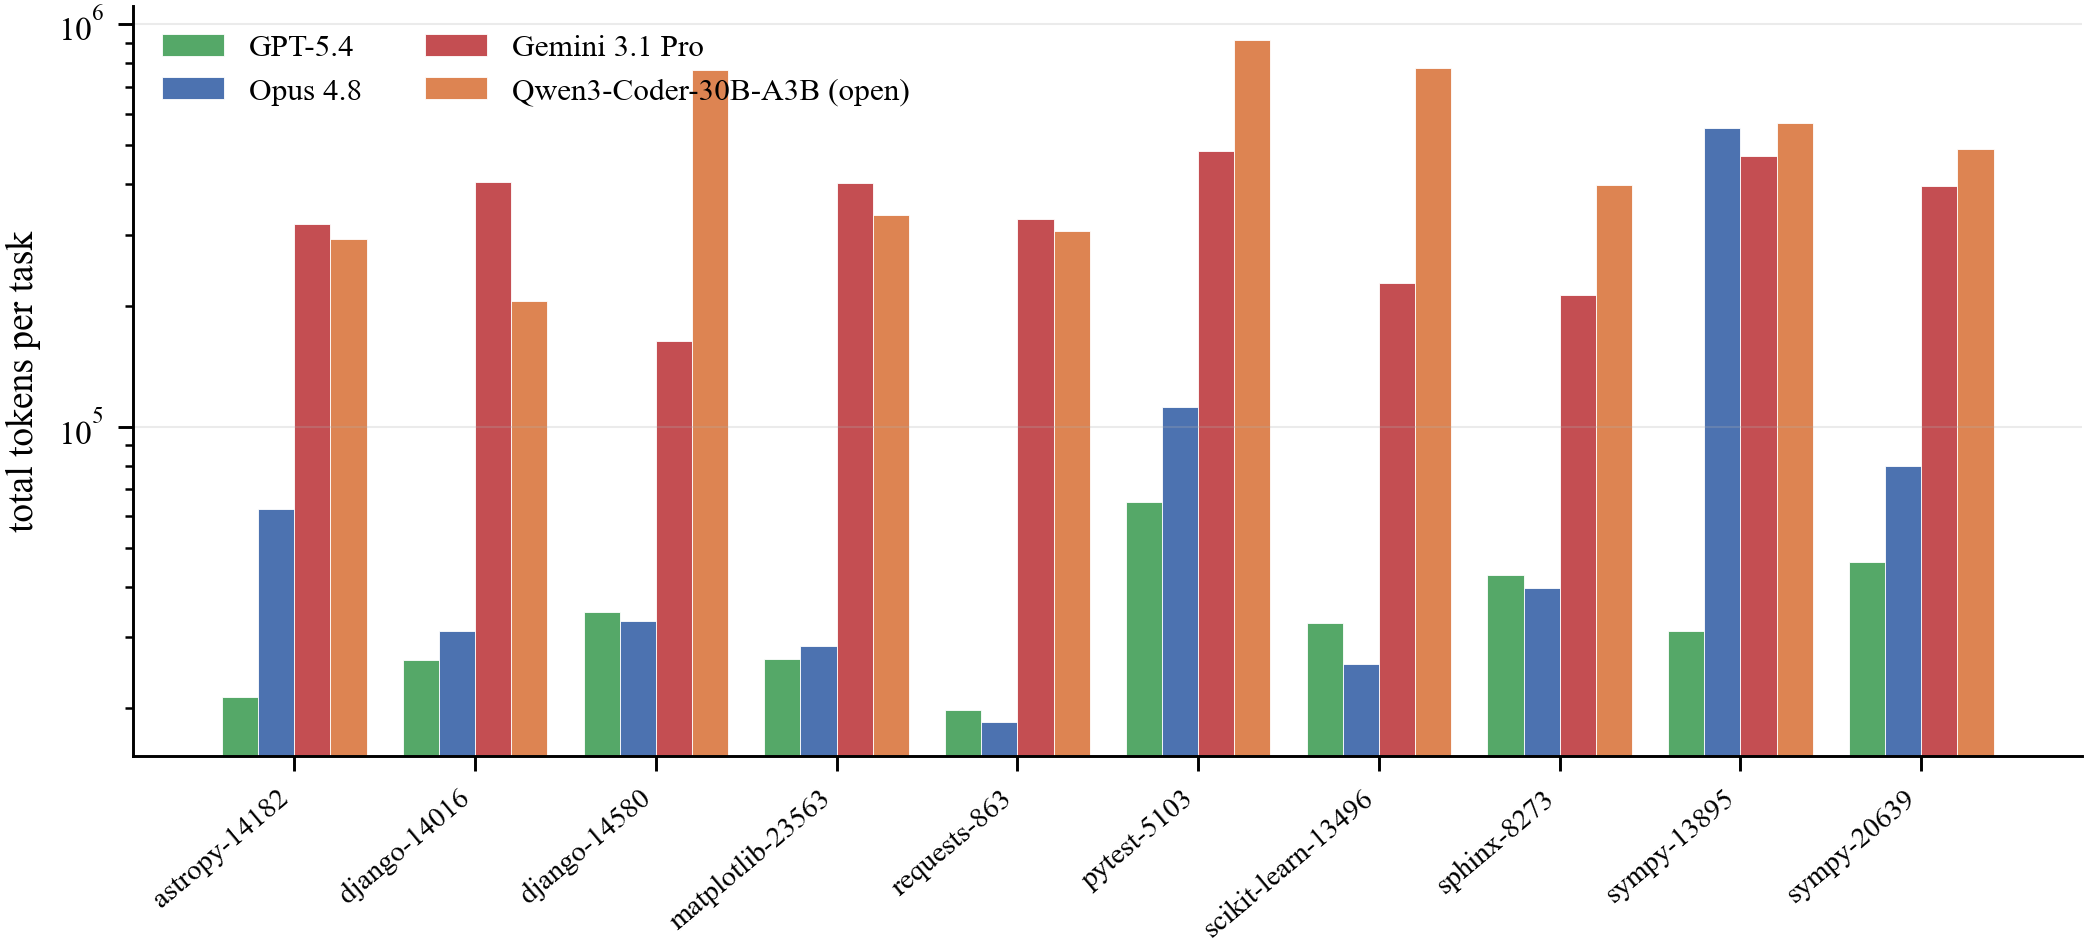
\includegraphics[width=0.5\linewidth]{figures/Figa1_sanity_tokens.png}
    \caption{Sanity check comparing total token consumption of frontier commercial
models (GPT-5.4, Claude Opus~4.8, and Gemini~3.1 Pro) with the
open-weight model Qwen3-Coder-30B-A3B on the same ten SWE-bench Lite
tasks using an identical mini-SWE-agent workflow. Although the
open-weight model generally consumes more tokens because of additional
tool retries and longer reasoning trajectories, all models remain within
the same $10^{5}$--$10^{6}$ tokens-per-task regime. This result supports
the assumption that software-engineering token demand is primarily
determined by the task and agent workflow, while model choice mainly
affects inference efficiency.
}
    \label{fig:placeholder}
\end{figure}

This sanity check does not imply identical token consumption across model
families. Instead, it demonstrates that the measured workload remains
within the same order of magnitude despite architectural and capability
differences, making the token-demand and throughput experiments
compatible for infrastructure-level analysis.

\section{Full Parameter Table}
\label{app:parameters}

\subsection*{A.1 Locked Assumptions}

See Section~\ref{sec:assumptions}, Table~\ref{tab:locked-assumptions}.

\subsection*{A.2 Scenario Matrix}

\begin{table}[ht]
\centering
\caption{Authoritative Scenario Matrix}
\label{tab:scenario-matrix}
\small
\begin{tabular}{@{}llrrrrrr@{}}
\hline
\textbf{Scenario} & \textbf{Mode} & \textbf{FTEs} & \textbf{Tok/Day} & \textbf{H100s} & \textbf{Power} & \textbf{Capex} & \textbf{AI \$/FTE-yr} \\
\hline
Conservative & Agentic & 2.4M & 9.6T & $\sim$33,700 & 36.8 MW & \$552M & $\sim$\$9,020 \\
Central & Agentic & 7.2M & 28.8T & $\sim$101,000 & 110 MW & \$1.65B & $\sim$\$9,020 \\
Aggressive & Agentic & 19.2M & 76.8T & $\sim$269,000 & 293 MW & \$4.40B & $\sim$\$9,020 \\
Conservative & Copilot & 2.4M & 288B & $\sim$9,600 & 12.3 MW & \$184M & $\sim$\$120 \\
Central & Copilot & 7.2M & 864B & $\sim$28,800 & 36.7 MW & \$551M & $\sim$\$120 \\
Aggressive & Copilot & 19.2M & 2.30T & $\sim$76,800 & 97.9 MW & \$1.47B & $\sim$\$120 \\
\hline
\end{tabular}
\end{table}

\subsection*{A.3 Sensitivity Parameters}

\begin{table}[ht]
\centering
\caption{Sensitivity Parameter Ranges}
\label{tab:sensitivity-params}
\small
\begin{tabular}{@{}p{4.5cm}rrr p{4.5cm}@{}}
\hline
\textbf{Parameter} & \textbf{Low} & \textbf{Central} & \textbf{High} & \textbf{Impact on 30\% scenario daily token demand} \\
\hline
Global developer count & 19.6M & 24M & 28.7M & $\pm$20\% \\
Tokens per task & 1M & 2.25M & 3.5M & $-$56\% / +56\% \\
Tasks per FTE per day & 1 & 2 & 4 & $-$50\% / +100\% \\
H100 inference TDP & 700W & 700W & 1,275W & affects power, not token demand \\
Construction cost (\$/MW) & \$10M & \$15M & \$20M & affects capex, not token demand \\
Electricity price (\$/MWh) & \$40 & \$60 & \$100 & affects energy cost, not token demand \\
PUE & 1.30 & 1.56 & 1.70 & $\pm$9\% on facility power \\
\hline
\end{tabular}
\end{table}

% ─────────────────────────────────────────────────────────────────────────────
\section{Sensitivity Analysis}
\label{app:sensitivity}

[Tornado charts and sensitivity tables to be added. See Section~\ref{sec:assumptions}
and Appendix~\ref{app:parameters} Table~\ref{tab:sensitivity-params} for the parameter
ranges used.]

The dominant uncertainty sources in order of impact on aggregate daily token demand are:
\begin{enumerate}
  \item Tokens per task ($\pm$56\% at the 30\% central scenario)
  \item Tasks per FTE per day ($-$50\% / +100\%)
  \item Global developer count ($\pm$20\%)
  \item Substitution rate (the primary scenario variable)
\end{enumerate}

Infrastructure cost sensitivity (30\% scenario):
\begin{itemize}
  \item Construction cost: \$1.65B $\pm$ \$550M (at \$10M--\$20M/MW range)
  \item Annual energy cost: \$38M--\$96M (at \$40--\$100/MWh range)
  \item Facility power: 100--120 MW (at PUE 1.30--1.70 range)
\end{itemize}


% ─────────────────────────────────────────────────────────────────────────────
\section{Timeline of AI Engineering Tools (2020--2025)}
\label{app:timeline}

\begin{longtable}{@{}p{1.2cm}p{5.5cm}p{5.5cm}@{}}
\hline
\textbf{Year} & \textbf{Event} & \textbf{Significance} \\
\hline
\endhead
\hline
\endfoot
2021 & GitHub Copilot technical preview (OpenAI Codex) & First mainstream AI code completion tool \\
2022 & GitHub Copilot general availability & 20M+ eventual users; establishes copilot-augmented mode \\
2022 & ChatGPT release (November) & Demonstrates frontier LLM capability for general-purpose coding assistance \\
2023 & GPT-4 release (March) & Frontier-class performance on coding benchmarks; API-accessible \\
2023 & Devin 1.0 announcement (Cognition AI) & First public demonstration of fully agentic software engineering \\
2023 & Claude 1/2 (Anthropic); expanded context windows & Long-context models enable full codebase loading in agentic tasks \\
2024 & SWE-bench introduced & Empirical benchmark for agentic coding; enables rigorous capability comparison \\
2024 & NVIDIA H100 widespread deployment & Hardware platform for frontier AI inference at scale \\
2024 & Cursor, Windsurf, Codeium reach scale & IDE-native agentic coding tools enter mainstream enterprise use \\
2024 & Microsoft--Constellation TMI-1 PPA & First hyperscaler nuclear PPA; establishes market-clearing price for 24/7 clean AI power \\
2025 & Devin 2.0 (13.86\% SWE-bench) & Best public agentic benchmark; establishes current capability frontier \\
2025 & NVIDIA GB200 NVL72 deployment begins & Blackwell generation: 40$\times$ rack density improvement over H100 air-cooled \\
2025 & Claude Code, OpenAI Operator class tools & Agentic coding agents integrated into developer workflows at enterprise scale \\
2025 & Amazon--Energy Northwest SMR announcement & Hyperscaler commitment to next-generation nuclear for AI load \\
\end{longtable}

\end{document}
